% Options for packages loaded elsewhere
% Options for packages loaded elsewhere
\PassOptionsToPackage{unicode}{hyperref}
\PassOptionsToPackage{hyphens}{url}
%
\documentclass[
  ignorenonframetext,
  aspectratio=169,
  russian,
]{beamer}
\newif\ifbibliography
\usepackage{pgfpages}
\setbeamertemplate{caption}[numbered]
\setbeamertemplate{caption label separator}{: }
\setbeamercolor{caption name}{fg=normal text.fg}
\beamertemplatenavigationsymbolshorizontal
% remove section numbering
\setbeamertemplate{part page}{
  \centering
  \begin{beamercolorbox}[sep=16pt,center]{part title}
    \usebeamerfont{part title}\insertpart\par
  \end{beamercolorbox}
}
\setbeamertemplate{section page}{
  \centering
  \begin{beamercolorbox}[sep=12pt,center]{section title}
    \usebeamerfont{section title}\insertsection\par
  \end{beamercolorbox}
}
\setbeamertemplate{subsection page}{
  \centering
  \begin{beamercolorbox}[sep=8pt,center]{subsection title}
    \usebeamerfont{subsection title}\insertsubsection\par
  \end{beamercolorbox}
}
% Prevent slide breaks in the middle of a paragraph
\widowpenalties 1 10000
\raggedbottom
\AtBeginPart{
  \frame{\partpage}
}
\AtBeginSection{
  \ifbibliography
  \else
    \frame{\sectionpage}
  \fi
}
\AtBeginSubsection{
  \frame{\subsectionpage}
}
\usepackage{iftex}
\ifPDFTeX
  \usepackage[T1]{fontenc}
  \usepackage[utf8]{inputenc}
  \usepackage{textcomp} % provide euro and other symbols
\else % if luatex or xetex
  \usepackage{unicode-math} % this also loads fontspec
  \defaultfontfeatures{Scale=MatchLowercase}
  \defaultfontfeatures[\rmfamily]{Ligatures=TeX,Scale=1}
\fi
\usepackage{lmodern}

\ifPDFTeX\else
  % xetex/luatex font selection
\fi
% Use upquote if available, for straight quotes in verbatim environments
\IfFileExists{upquote.sty}{\usepackage{upquote}}{}
\IfFileExists{microtype.sty}{% use microtype if available
  \usepackage[]{microtype}
  \UseMicrotypeSet[protrusion]{basicmath} % disable protrusion for tt fonts
}{}

\usepackage{color}
\usepackage{fancyvrb}
\newcommand{\VerbBar}{|}
\newcommand{\VERB}{\Verb[commandchars=\\\{\}]}
\DefineVerbatimEnvironment{Highlighting}{Verbatim}{commandchars=\\\{\}}
% Add ',fontsize=\small' for more characters per line
\usepackage{framed}
\definecolor{shadecolor}{RGB}{241,243,245}
\newenvironment{Shaded}{\begin{snugshade}}{\end{snugshade}}
\newcommand{\AlertTok}[1]{\textcolor[rgb]{0.68,0.00,0.00}{#1}}
\newcommand{\AnnotationTok}[1]{\textcolor[rgb]{0.37,0.37,0.37}{#1}}
\newcommand{\AttributeTok}[1]{\textcolor[rgb]{0.40,0.45,0.13}{#1}}
\newcommand{\BaseNTok}[1]{\textcolor[rgb]{0.68,0.00,0.00}{#1}}
\newcommand{\BuiltInTok}[1]{\textcolor[rgb]{0.00,0.23,0.31}{#1}}
\newcommand{\CharTok}[1]{\textcolor[rgb]{0.13,0.47,0.30}{#1}}
\newcommand{\CommentTok}[1]{\textcolor[rgb]{0.37,0.37,0.37}{#1}}
\newcommand{\CommentVarTok}[1]{\textcolor[rgb]{0.37,0.37,0.37}{\textit{#1}}}
\newcommand{\ConstantTok}[1]{\textcolor[rgb]{0.56,0.35,0.01}{#1}}
\newcommand{\ControlFlowTok}[1]{\textcolor[rgb]{0.00,0.23,0.31}{\textbf{#1}}}
\newcommand{\DataTypeTok}[1]{\textcolor[rgb]{0.68,0.00,0.00}{#1}}
\newcommand{\DecValTok}[1]{\textcolor[rgb]{0.68,0.00,0.00}{#1}}
\newcommand{\DocumentationTok}[1]{\textcolor[rgb]{0.37,0.37,0.37}{\textit{#1}}}
\newcommand{\ErrorTok}[1]{\textcolor[rgb]{0.68,0.00,0.00}{#1}}
\newcommand{\ExtensionTok}[1]{\textcolor[rgb]{0.00,0.23,0.31}{#1}}
\newcommand{\FloatTok}[1]{\textcolor[rgb]{0.68,0.00,0.00}{#1}}
\newcommand{\FunctionTok}[1]{\textcolor[rgb]{0.28,0.35,0.67}{#1}}
\newcommand{\ImportTok}[1]{\textcolor[rgb]{0.00,0.46,0.62}{#1}}
\newcommand{\InformationTok}[1]{\textcolor[rgb]{0.37,0.37,0.37}{#1}}
\newcommand{\KeywordTok}[1]{\textcolor[rgb]{0.00,0.23,0.31}{\textbf{#1}}}
\newcommand{\NormalTok}[1]{\textcolor[rgb]{0.00,0.23,0.31}{#1}}
\newcommand{\OperatorTok}[1]{\textcolor[rgb]{0.37,0.37,0.37}{#1}}
\newcommand{\OtherTok}[1]{\textcolor[rgb]{0.00,0.23,0.31}{#1}}
\newcommand{\PreprocessorTok}[1]{\textcolor[rgb]{0.68,0.00,0.00}{#1}}
\newcommand{\RegionMarkerTok}[1]{\textcolor[rgb]{0.00,0.23,0.31}{#1}}
\newcommand{\SpecialCharTok}[1]{\textcolor[rgb]{0.37,0.37,0.37}{#1}}
\newcommand{\SpecialStringTok}[1]{\textcolor[rgb]{0.13,0.47,0.30}{#1}}
\newcommand{\StringTok}[1]{\textcolor[rgb]{0.13,0.47,0.30}{#1}}
\newcommand{\VariableTok}[1]{\textcolor[rgb]{0.07,0.07,0.07}{#1}}
\newcommand{\VerbatimStringTok}[1]{\textcolor[rgb]{0.13,0.47,0.30}{#1}}
\newcommand{\WarningTok}[1]{\textcolor[rgb]{0.37,0.37,0.37}{\textit{#1}}}

\usepackage{longtable,booktabs,array}
\newcounter{none} % for unnumbered tables
\usepackage{calc} % for calculating minipage widths
\usepackage{caption}
% Make caption package work with longtable
\makeatletter
\def\fnum@table{\tablename~\thetable}
\makeatother
\usepackage{graphicx}
\makeatletter
\newsavebox\pandoc@box
\newcommand*\pandocbounded[1]{% scales image to fit in text height/width
  \sbox\pandoc@box{#1}%
  \Gscale@div\@tempa{\textheight}{\dimexpr\ht\pandoc@box+\dp\pandoc@box\relax}%
  \Gscale@div\@tempb{\linewidth}{\wd\pandoc@box}%
  \ifdim\@tempb\p@<\@tempa\p@\let\@tempa\@tempb\fi% select the smaller of both
  \ifdim\@tempa\p@<\p@\scalebox{\@tempa}{\usebox\pandoc@box}%
  \else\usebox{\pandoc@box}%
  \fi%
}
% Set default figure placement to htbp
\def\fps@figure{htbp}
\makeatother



\ifLuaTeX
\usepackage[bidi=basic,shorthands=off,provide=*]{babel}
\else
\usepackage[bidi=default,shorthands=off,provide=*]{babel}
\fi
\ifLuaTeX
  \usepackage{selnolig} % disable illegal ligatures
\fi


\setlength{\emergencystretch}{3em} % prevent overfull lines

\providecommand{\tightlist}{%
  \setlength{\itemsep}{0pt}\setlength{\parskip}{0pt}}



 

\usepackage[]{csquotes}

\IfFileExists{plex-otf.sty}{
  %% Full TeXlive
  % \usepackage[%
  %   % math,
  %   RM={Scale=0.94},SS={Scale=0.94},SScon={Scale=0.94},TT={Scale=MatchLowercase,FakeStretch=0.9},DefaultFeatures={Ligatures=Common}
  % ]{plex-otf}
}{
  %% TinyTeX
  \usepackage{libertine}
}

%%% Load theme
% https://deic.uab.cat/~iblanes/beamer_gallery/
\IfFileExists{beamerthemegotham.sty}{
  %% Full TeXlive
  \usetheme{gotham}
  \gothamset{
    numbering=totalpagenumber,
    parttocframe default=off,
    sectiontocframe default=off,
    subsectiontocframe default=off,
  }
}{
  %% TinyTeX
  \usetheme{Madrid}
}
\makeatletter
\@ifpackageloaded{caption}{}{\usepackage{caption}}
\AtBeginDocument{%
\ifdefined\contentsname
  \renewcommand*\contentsname{Содержание}
\else
  \newcommand\contentsname{Содержание}
\fi
\ifdefined\listfigurename
  \renewcommand*\listfigurename{Список иллюстраций}
\else
  \newcommand\listfigurename{Список иллюстраций}
\fi
\ifdefined\listtablename
  \renewcommand*\listtablename{Список таблиц}
\else
  \newcommand\listtablename{Список таблиц}
\fi
\ifdefined\figurename
  \renewcommand*\figurename{Рисунок}
\else
  \newcommand\figurename{Рисунок}
\fi
\ifdefined\tablename
  \renewcommand*\tablename{Таблица}
\else
  \newcommand\tablename{Таблица}
\fi
}
\@ifpackageloaded{float}{}{\usepackage{float}}
\floatstyle{ruled}
\@ifundefined{c@chapter}{\newfloat{codelisting}{h}{lop}}{\newfloat{codelisting}{h}{lop}[chapter]}
\floatname{codelisting}{Список}
\newcommand*\listoflistings{\listof{codelisting}{Листинги}}
\makeatother
\makeatletter
\makeatother
\makeatletter
\@ifpackageloaded{caption}{}{\usepackage{caption}}
\@ifpackageloaded{subcaption}{}{\usepackage{subcaption}}
\makeatother

\usepackage{bookmark}
\IfFileExists{xurl.sty}{\usepackage{xurl}}{} % add URL line breaks if available
\urlstyle{same}
% fallback for those not using the hyperref driver hyperxmp:
\makeatletter
\@ifundefined{xmpquote}{\newcommand{\xmpquote}[1]{#1}}{}
\makeatother
\hypersetup{
  pdftitle={Лабораторная работа №1},
  pdfauthor={Кудякова София Андреевна},
  pdflang={ru},
  hidelinks,
  pdfcreator={LaTeX via pandoc}}


\title{\texorpdfstring{Лабораторная работа №1}{Лабораторная работа №1}}
\subtitle{\texorpdfstring{Работа с Git и моделирование экспоненциального
роста}{Работа с Git и моделирование экспоненциального роста}}
\author{Кудякова София Андреевна}
\date{2026-08-25}

\begin{document}
\frame{\titlepage}

\renewcommand*\contentsname{Содержание}
\begin{frame}[allowframebreaks]
  \frametitle{Содержание}
  \setcounter{tocdepth}{1}
  \tableofcontents
\end{frame}
\setcounter{tocdepth}{1}
\tableofcontents
}

\section{Вводная
часть}\label{ux432ux432ux43eux434ux43dux430ux44f-ux447ux430ux441ux442ux44c}

\begin{frame}{Актуальность}
\protect\phantomsection\label{ux430ux43aux442ux443ux430ux43bux44cux43dux43eux441ux442ux44c}
\begin{itemize}[<+->]
\tightlist
\item
  Git используется для контроля версий и синхронизации проекта
\item
  DrWatson обеспечивает структуру и воспроизводимость вычислений
\item
  Julia используется для численного моделирования
\item
  Literate и Quarto позволяют автоматизировать подготовку документации
\end{itemize}
\end{frame}

\begin{frame}{Цель и задачи}
\protect\phantomsection\label{ux446ux435ux43bux44c-ux438-ux437ux430ux434ux430ux447ux438}
\textbf{Цель:} настроить рабочее окружение и исследовать модель
экспоненциального роста.

\textbf{Задачи:}

\begin{itemize}[<+->]
\tightlist
\item
  настроить Git и SSH;
\item
  создать проект DrWatson;
\item
  реализовать модель на Julia;
\item
  выполнить моделирование;
\item
  провести параметрическое исследование;
\item
  подготовить Jupyter Notebook и Quarto-отчёт.
\end{itemize}
\end{frame}

\begin{frame}{Модель экспоненциального роста}
\protect\phantomsection\label{ux43cux43eux434ux435ux43bux44c-ux44dux43aux441ux43fux43eux43dux435ux43dux446ux438ux430ux43bux44cux43dux43eux433ux43e-ux440ux43eux441ux442ux430}
Дифференциальное уравнение:

\[
\frac{du}{dt}=\alpha u
\]

Начальное условие:

\[
u(0)=u_0
\]

Аналитическое решение:

\[
u(t)=u_0e^{\alpha t}
\]
\end{frame}

\section{Выполнение}\label{ux432ux44bux43fux43eux43bux43dux435ux43dux438ux435}

\begin{frame}{Настройка Git}
\protect\phantomsection\label{ux43dux430ux441ux442ux440ux43eux439ux43aux430-git}
\begin{itemize}[<+->]
\tightlist
\item
  Настроены имя и электронная почта пользователя
\item
  Настроены параметры отображения путей и окончания строк
\item
  Настроен базовый branch по умолчанию
\end{itemize}

\begin{figure}

\centering{

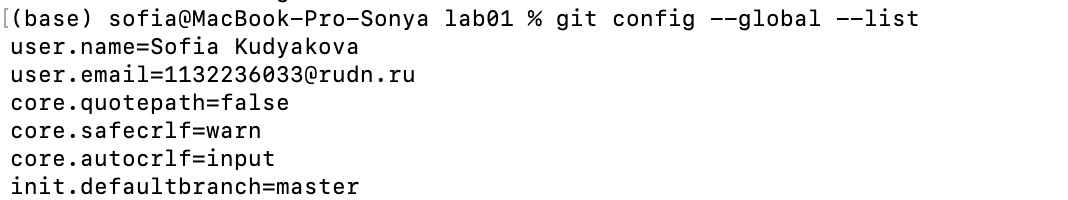
\includegraphics[width=0.7\linewidth,height=\textheight,keepaspectratio]{image/1.png}

}

\caption{\label{fig-001}Настройка Git}

\end{figure}%
\end{frame}

\begin{frame}{Настройка SSH-доступа}
\protect\phantomsection\label{ux43dux430ux441ux442ux440ux43eux439ux43aux430-ssh-ux434ux43eux441ux442ux443ux43fux430}
\begin{itemize}[<+->]
\tightlist
\item
  Создан SSH-ключ по алгоритму Ed25519
\item
  Открытая часть ключа добавлена в удалённый репозиторий
\item
  Проверено соединение --- аутентификация настроена корректно
\end{itemize}

\begin{figure}

\centering{

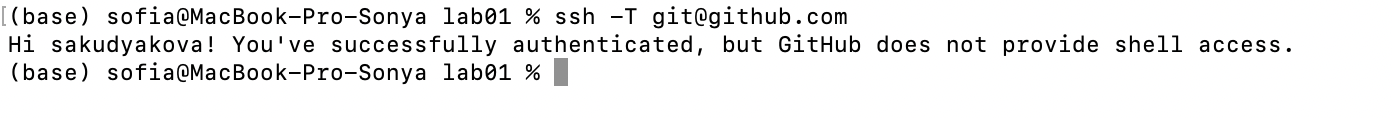
\includegraphics[width=0.7\linewidth,height=\textheight,keepaspectratio]{image/2.png}

}

\caption{\label{fig-002}Настройка SSH-доступа}

\end{figure}%
\end{frame}

\begin{frame}{Настройка GitVerse}
\protect\phantomsection\label{ux43dux430ux441ux442ux440ux43eux439ux43aux430-gitverse}
\begin{itemize}[<+->]
\tightlist
\item
  Настроен GitVerse как дополнительная платформа хранения
\item
  Проверен доступ к репозиторию
\item
  Настроено взаимодействие через Git
\end{itemize}

\begin{figure}

\centering{

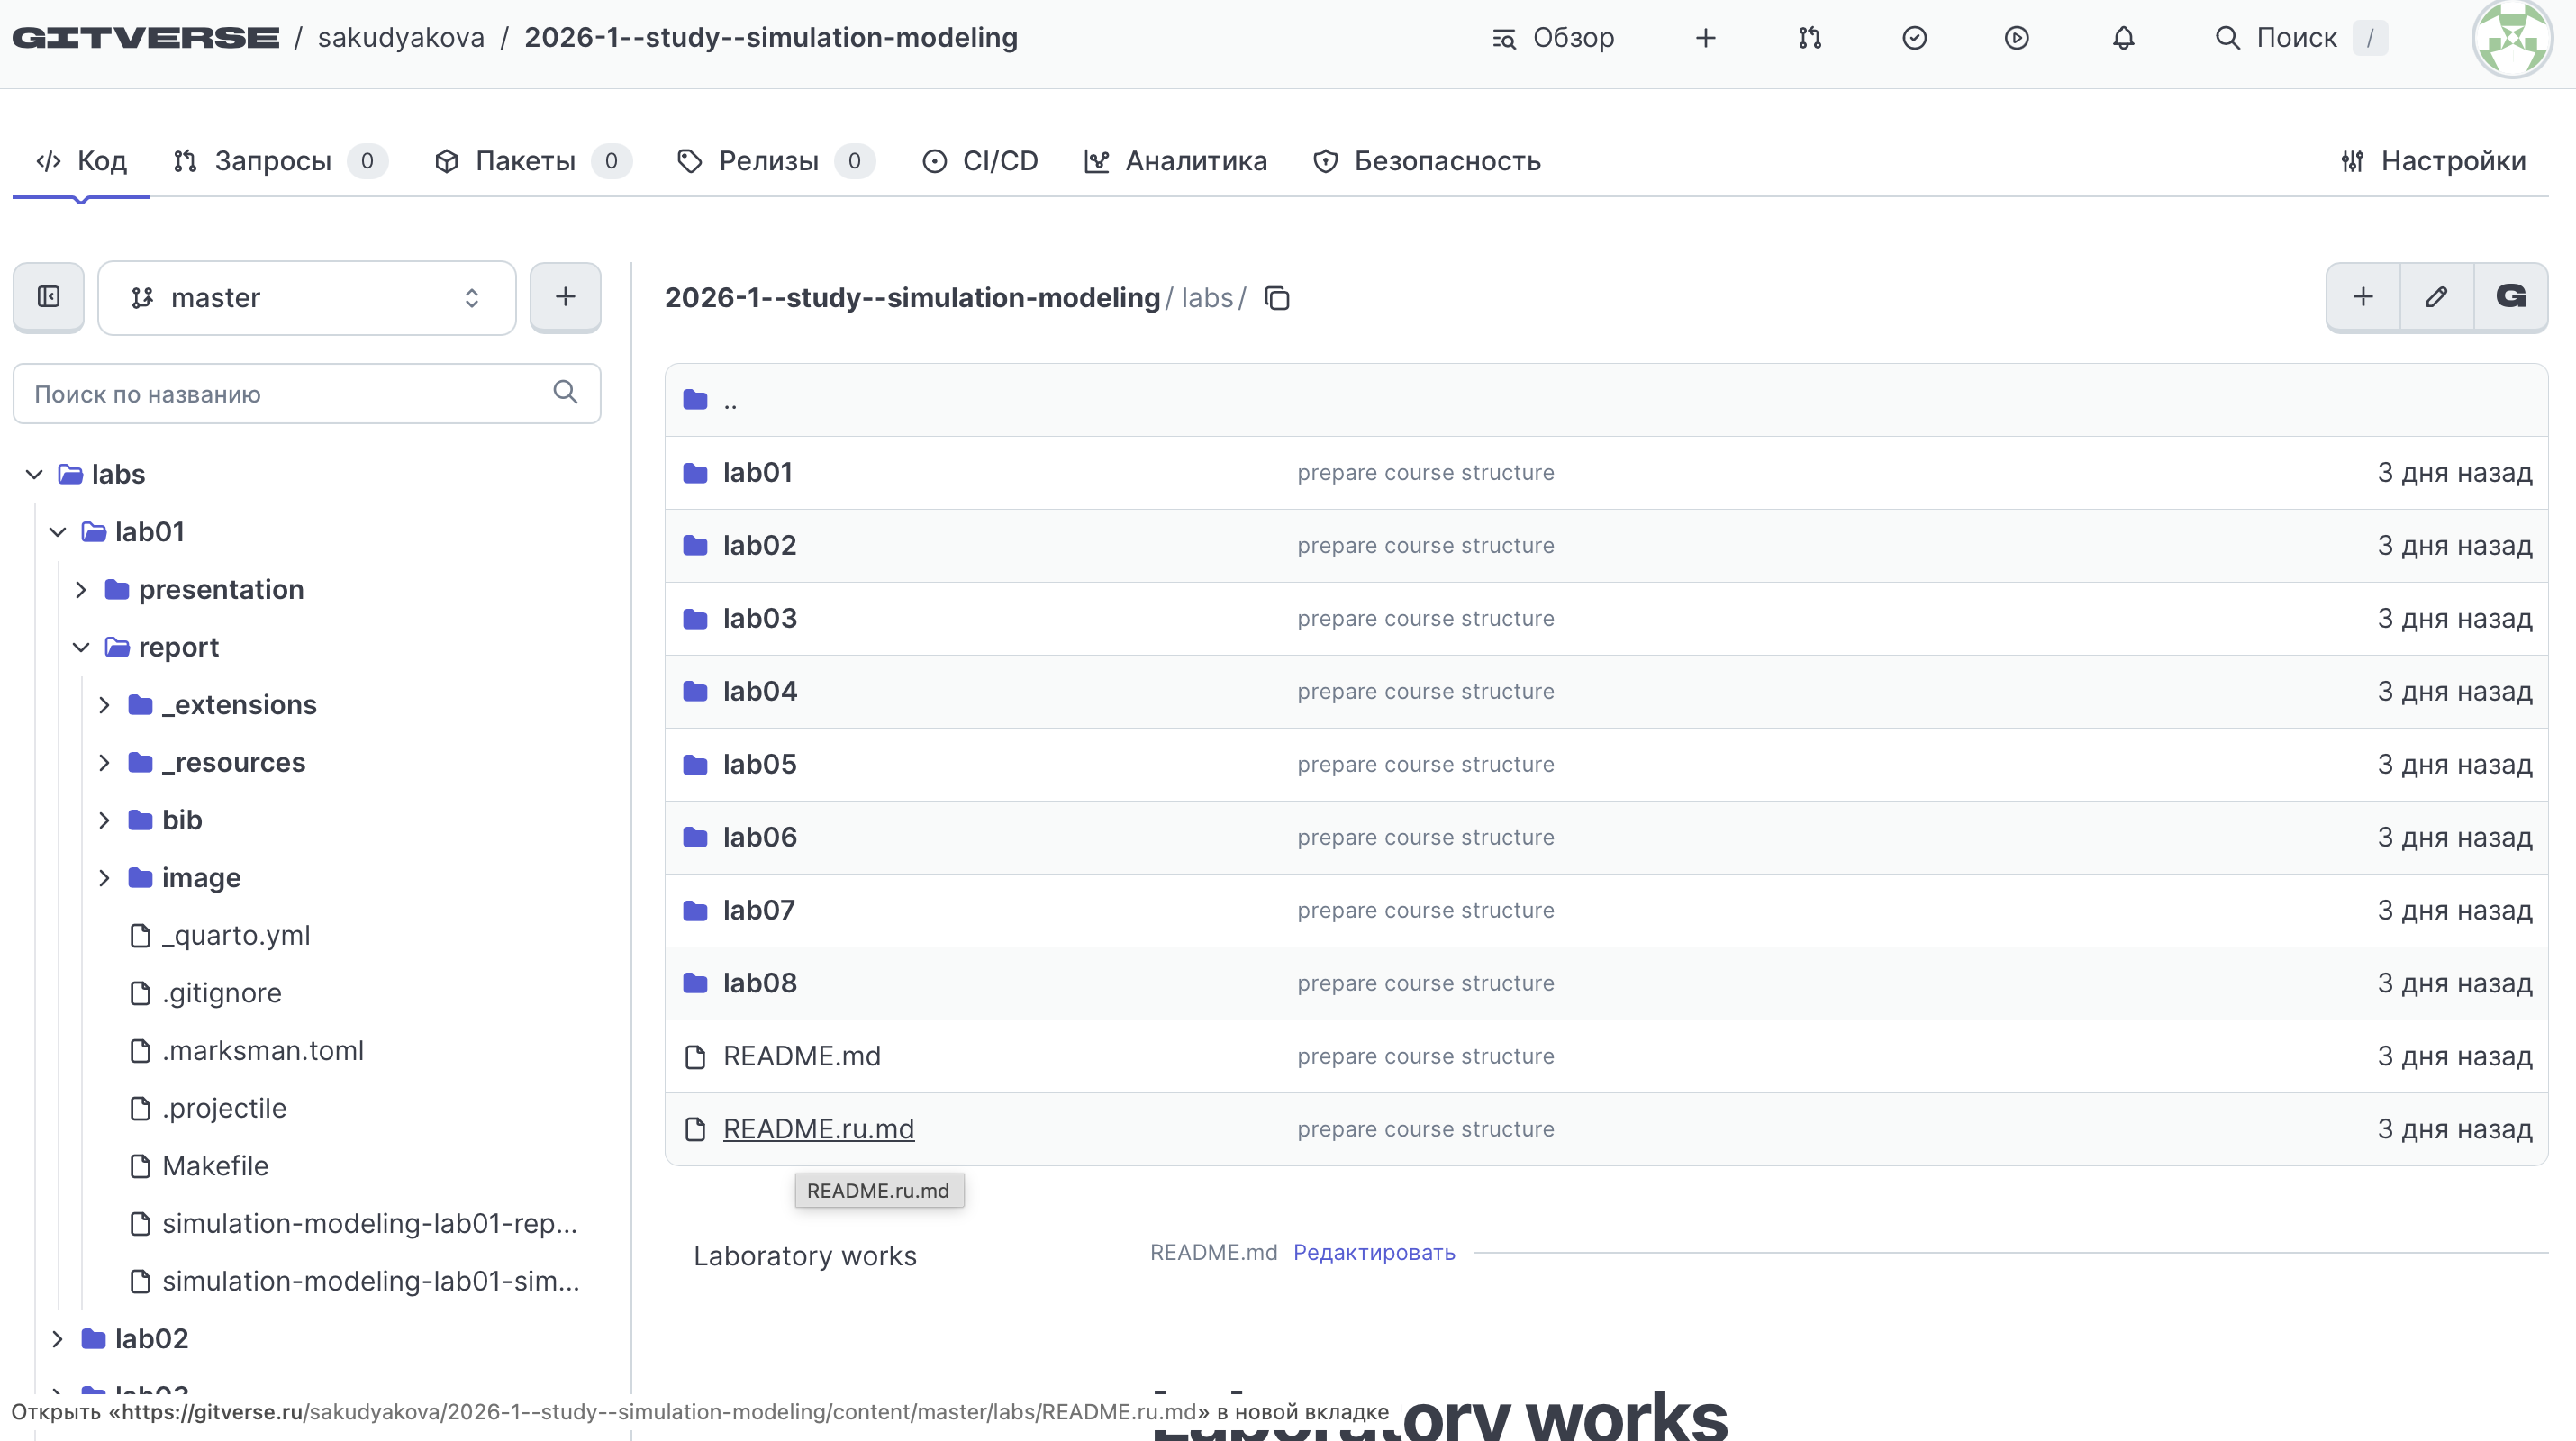
\includegraphics[width=0.7\linewidth,height=\textheight,keepaspectratio]{image/333.png}

}

\caption{\label{fig-333}}

\end{figure}%
\end{frame}

\begin{frame}{Рабочее пространство курса}
\protect\phantomsection\label{ux440ux430ux431ux43eux447ux435ux435-ux43fux440ux43eux441ux442ux440ux430ux43dux441ux442ux432ux43e-ux43aux443ux440ux441ux430}
\begin{itemize}[<+->]
\tightlist
\item
  Создан каталог лабораторной работы lab01
\item
  project --- вычисления и результаты
\item
  report --- документация
\end{itemize}

\begin{figure}

\centering{

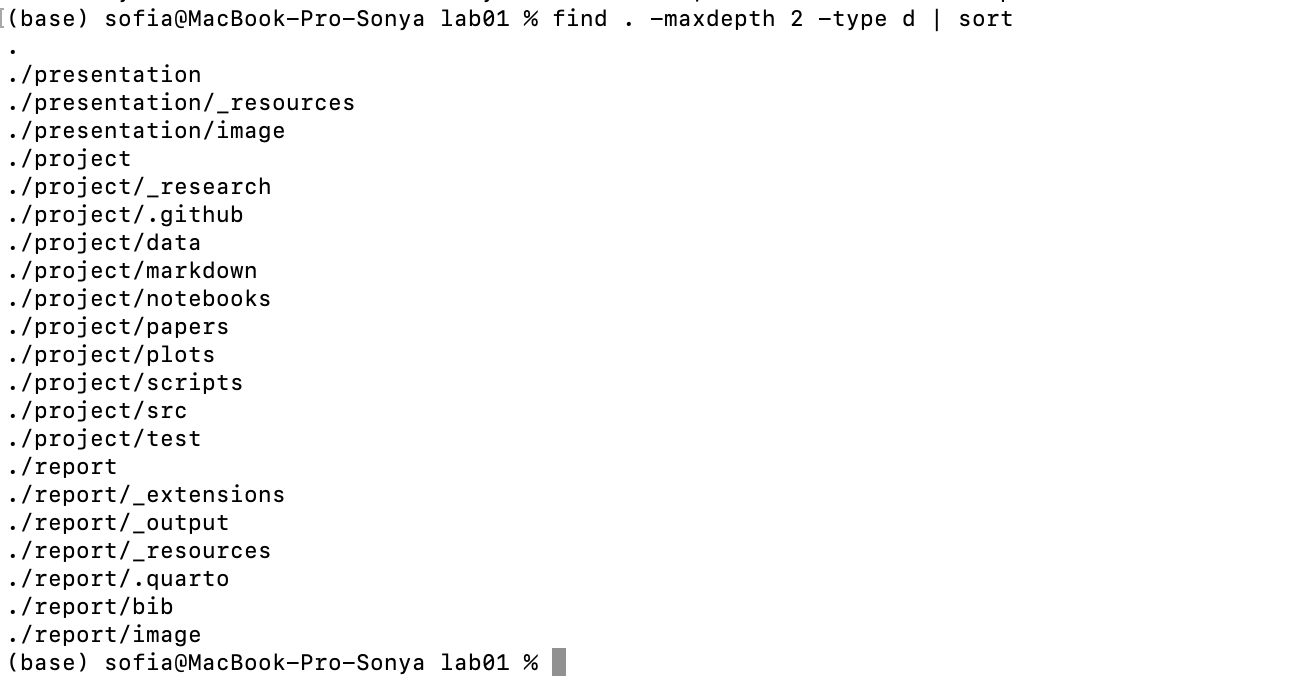
\includegraphics[width=0.7\linewidth,height=\textheight,keepaspectratio]{image/3.png}

}

\caption{\label{fig-003}Создание рабочего пространства курса}

\end{figure}%
\end{frame}

\begin{frame}{Проект DrWatson}
\protect\phantomsection\label{ux43fux440ux43eux435ux43aux442-drwatson}
Основные каталоги проекта:

\begin{itemize}[<+->]
\tightlist
\item
  data/ --- данные
\item
  plots/ --- графики
\item
  scripts/ --- скрипты
\item
  notebooks/ --- Jupyter Notebook
\item
  markdown/ --- документы Quarto
\item
  src/ --- исходный код
\end{itemize}

\begin{figure}

\centering{

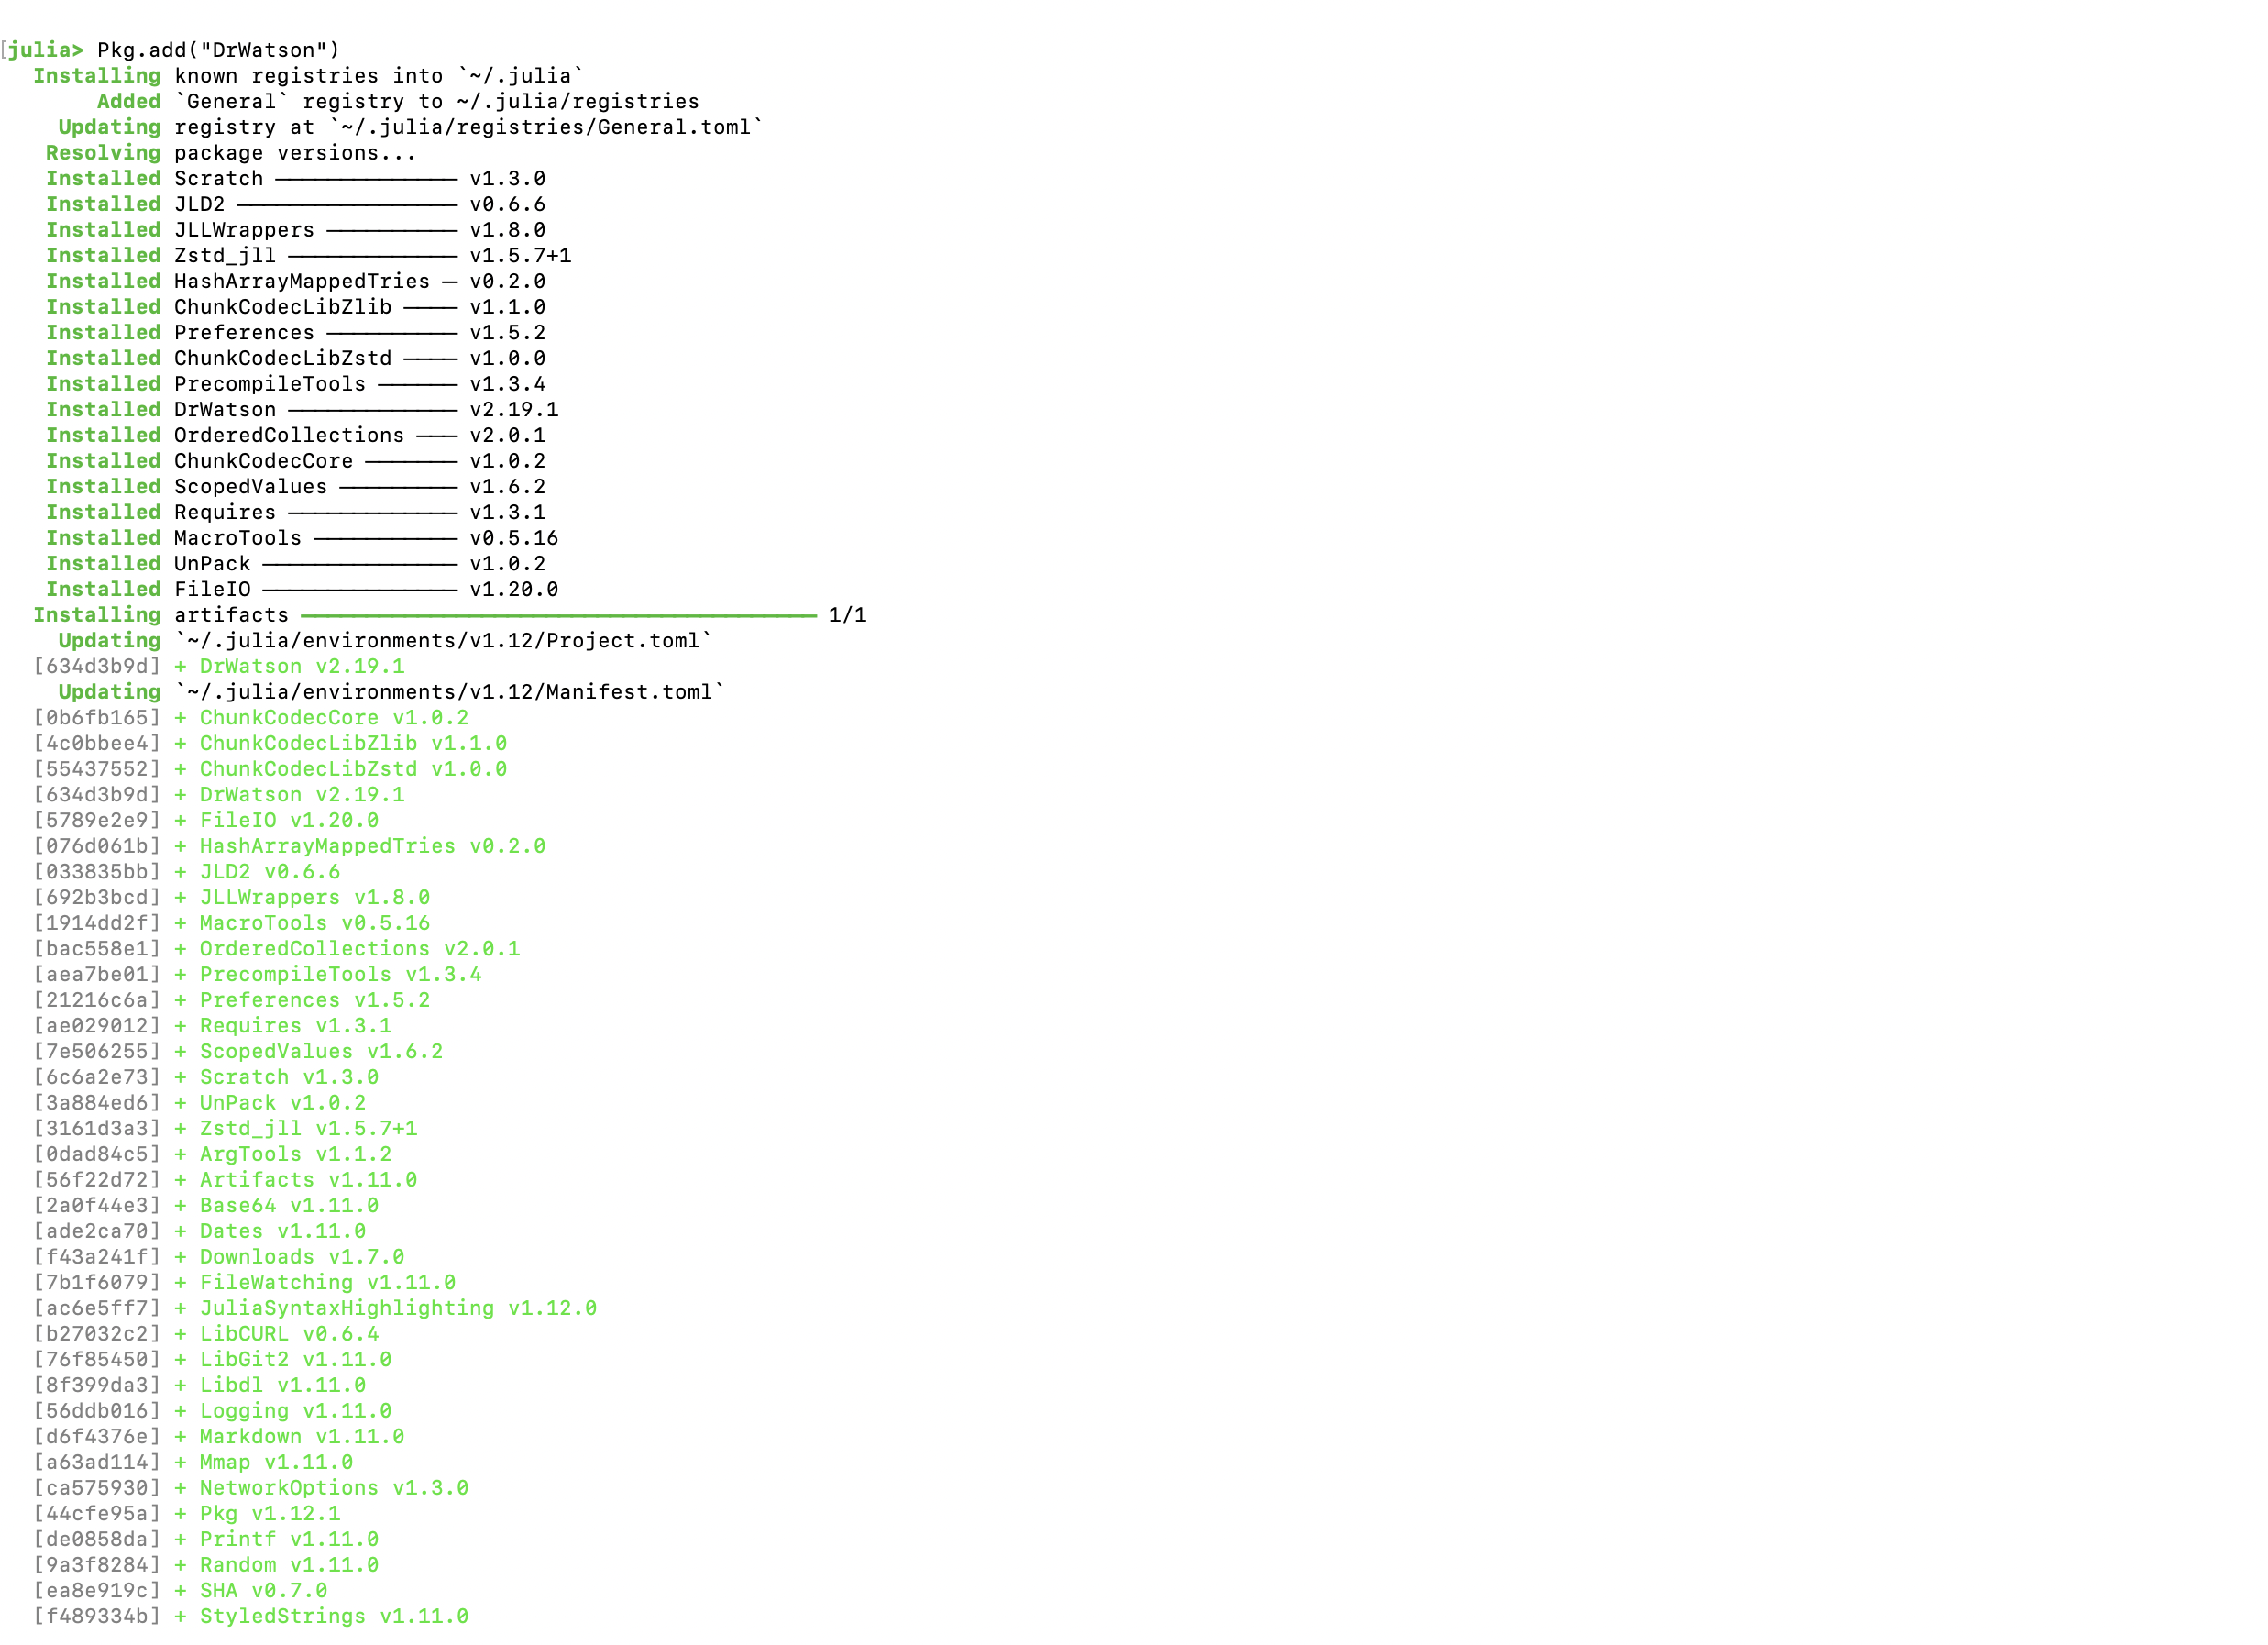
\includegraphics[width=0.7\linewidth,height=\textheight,keepaspectratio]{image/4.png}

}

\caption{\label{fig-004}DrWatson}

\end{figure}%
\end{frame}

\begin{frame}{Установка пакетов}
\protect\phantomsection\label{ux443ux441ux442ux430ux43dux43eux432ux43aux430-ux43fux430ux43aux435ux442ux43eux432}
Подключены основные пакеты:

\begin{itemize}[<+->]
\tightlist
\item
  DrWatson, DifferentialEquations, Plots
\item
  DataFrames, JLD2, Literate
\item
  IJulia, BenchmarkTools, Quarto
\end{itemize}

\begin{figure}

\centering{

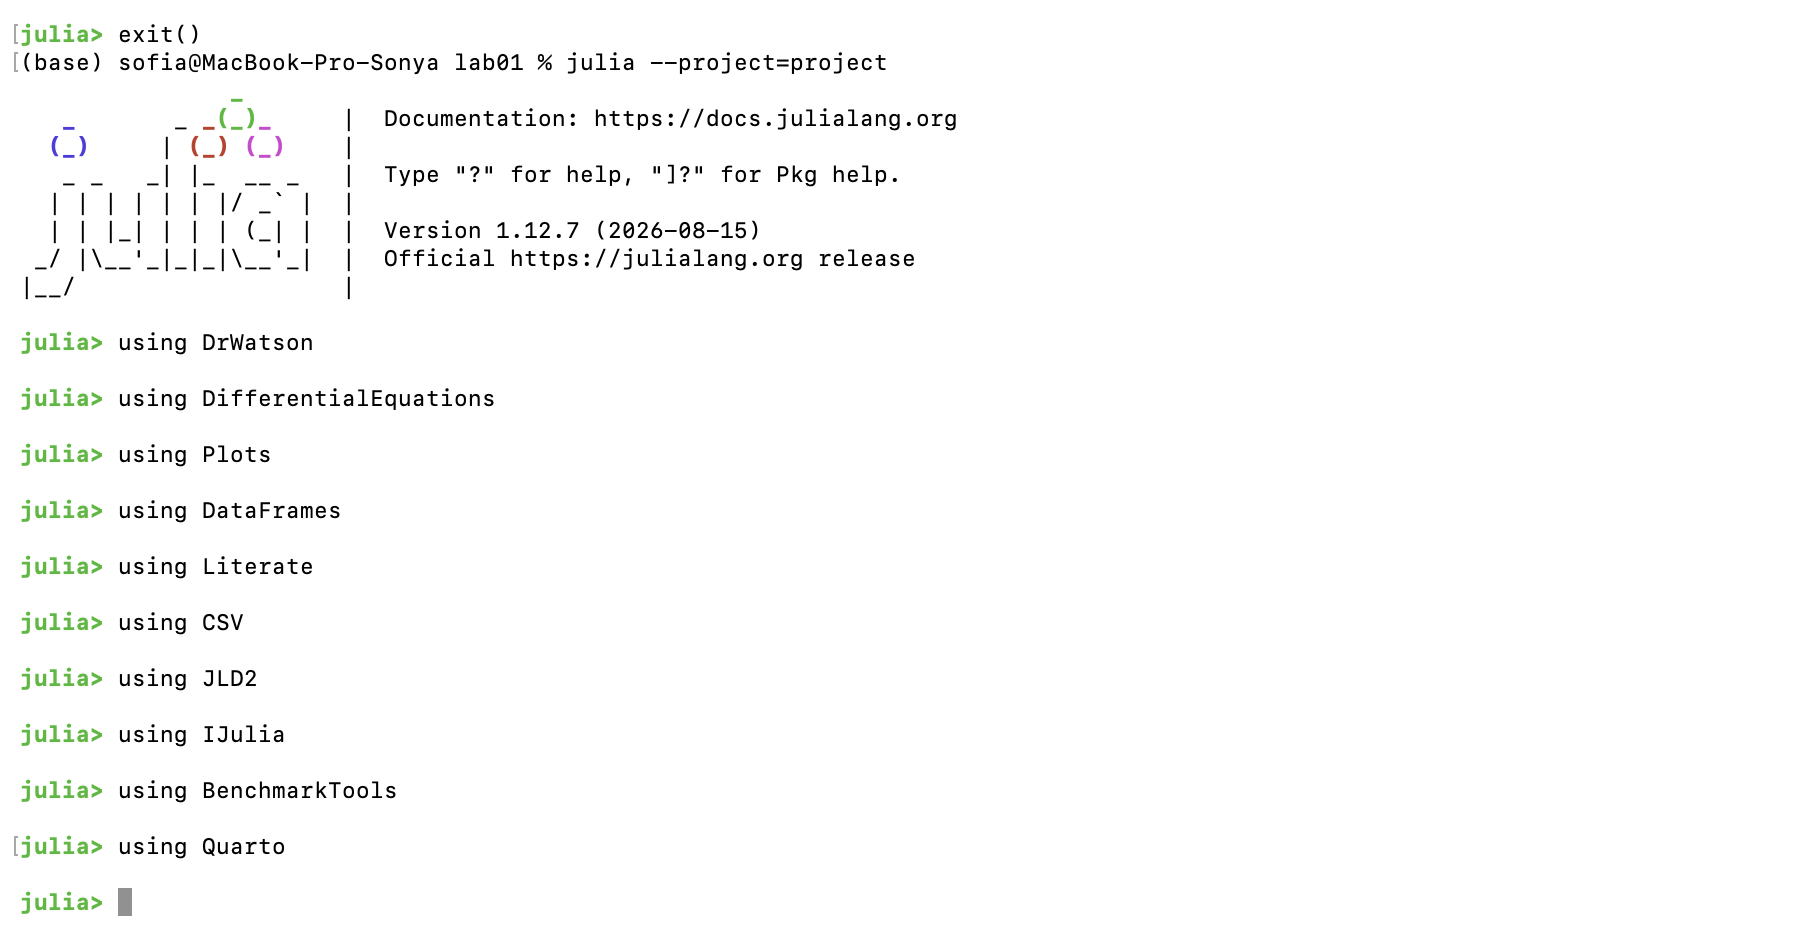
\includegraphics[width=0.7\linewidth,height=\textheight,keepaspectratio]{image/5.png}

}

\caption{\label{fig-005}Установка необходимых пакетов}

\end{figure}%
\end{frame}

\begin{frame}[fragile]{Проверка проекта}
\protect\phantomsection\label{ux43fux440ux43eux432ux435ux440ux43aux430-ux43fux440ux43eux435ux43aux442ux430}
\begin{itemize}[<+->]
\tightlist
\item
  Выполнена активация проекта через \texttt{@quickactivate}
\item
  Проверены основные пути проекта (root, data, scripts, plots)
\item
  Окружение настроено корректно
\end{itemize}

\begin{figure}

\centering{

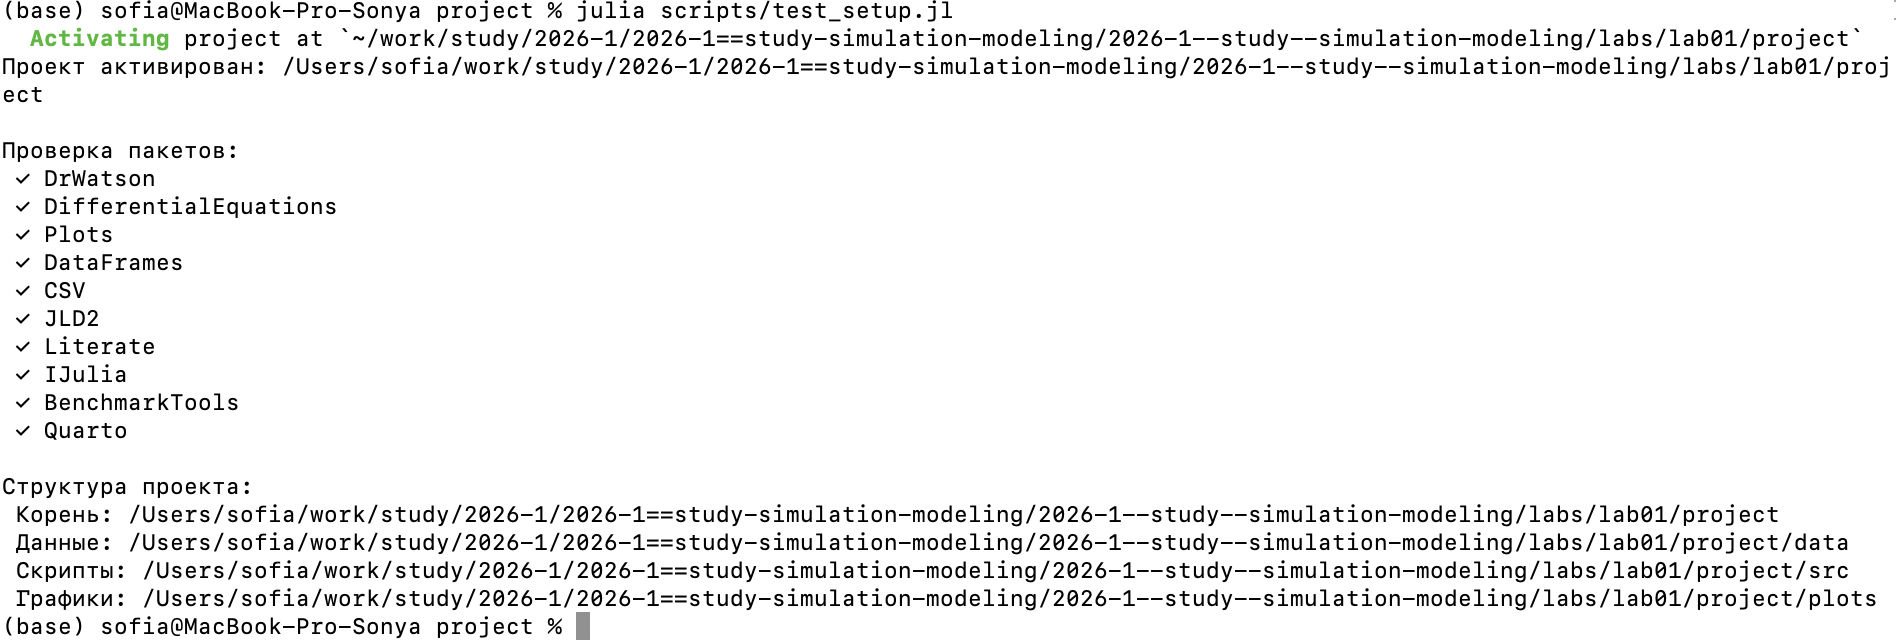
\includegraphics[width=0.7\linewidth,height=\textheight,keepaspectratio]{image/6.png}

}

\caption{\label{fig-006}Проверка проекта}

\end{figure}%
\end{frame}

\section{Моделирование}\label{ux43cux43eux434ux435ux43bux438ux440ux43eux432ux430ux43dux438ux435}

\begin{frame}[fragile]{Базовый эксперимент}
\protect\phantomsection\label{ux431ux430ux437ux43eux432ux44bux439-ux44dux43aux441ux43fux435ux440ux438ux43cux435ux43dux442}
Параметры:

\begin{Shaded}
\begin{Highlighting}[]
\NormalTok{u0 }\OperatorTok{=}\NormalTok{ [}\FloatTok{1.0}\NormalTok{]}
\NormalTok{α }\OperatorTok{=} \FloatTok{0.3}
\NormalTok{tspan }\OperatorTok{=}\NormalTok{ (}\FloatTok{0.0}\NormalTok{, }\FloatTok{10.0}\NormalTok{)}
\end{Highlighting}
\end{Shaded}

Численное решение выполняется методом \texttt{Tsit5()}.
\end{frame}

\begin{frame}{Результат моделирования}
\protect\phantomsection\label{ux440ux435ux437ux443ux43bux44cux442ux430ux442-ux43cux43eux434ux435ux43bux438ux440ux43eux432ux430ux43dux438ux44f}
При \(\alpha=0.3\) получена траектория экспоненциального роста.

\begin{figure}

\centering{

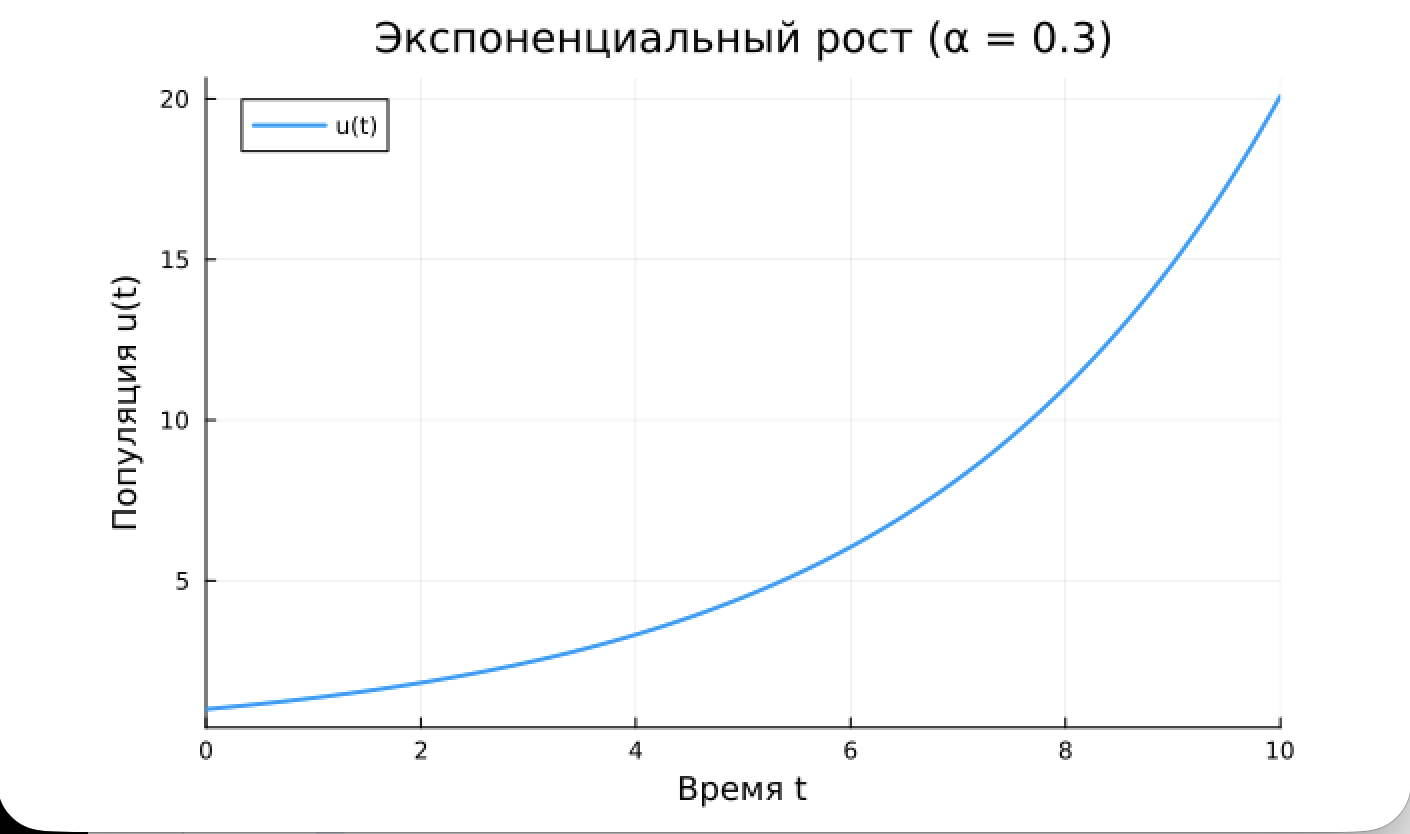
\includegraphics[width=0.7\linewidth,height=\textheight,keepaspectratio]{image/7.png}

}

\caption{\label{fig-007}График зависимости}

\end{figure}%
\end{frame}

\begin{frame}{Таблица результатов}
\protect\phantomsection\label{ux442ux430ux431ux43bux438ux446ux430-ux440ux435ux437ux443ux43bux44cux442ux430ux442ux43eux432}
Сформирована таблица моментов времени и значений \(u(t)\).

\begin{figure}

\centering{

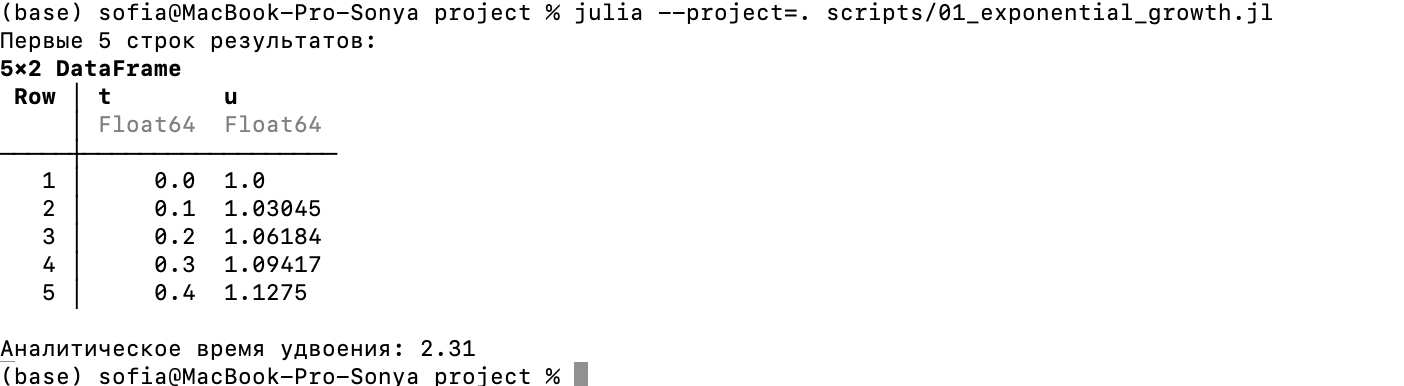
\includegraphics[width=0.7\linewidth,height=\textheight,keepaspectratio]{image/8.png}

}

\caption{\label{fig-008}Формирование таблицы результатов}

\end{figure}%
\end{frame}

\begin{frame}{Время удвоения}
\protect\phantomsection\label{ux432ux440ux435ux43cux44f-ux443ux434ux432ux43eux435ux43dux438ux44f}
Формула:

\[
T_2=\frac{\ln 2}{\alpha}
\]

Для \(\alpha=0.3\):

\[
T_2\approx2.31
\]

\begin{figure}

\centering{

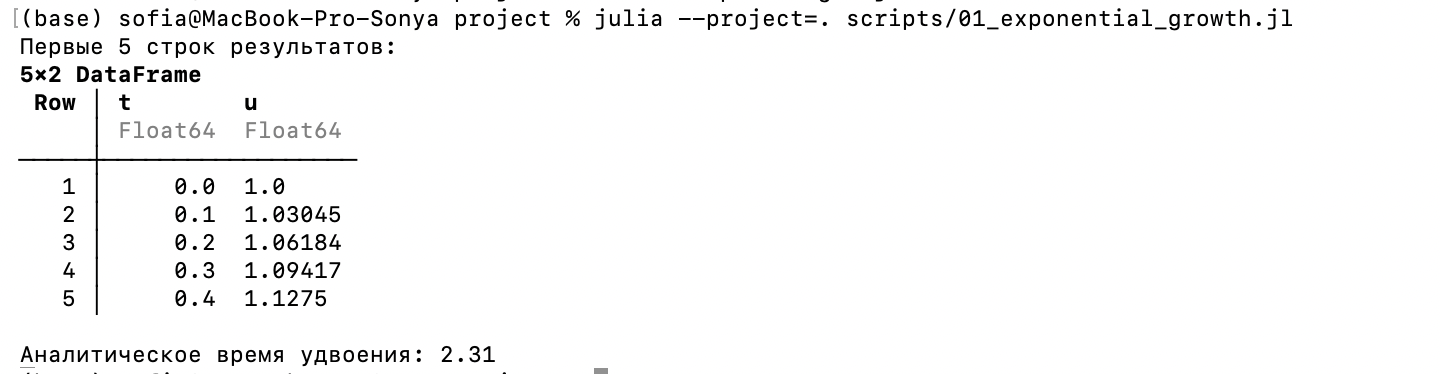
\includegraphics[width=0.7\linewidth,height=\textheight,keepaspectratio]{image/9.png}

}

\caption{\label{fig-009}Расчёт}

\end{figure}%
\end{frame}

\section{Литературное
программирование}\label{ux43bux438ux442ux435ux440ux430ux442ux443ux440ux43dux43eux435-ux43fux440ux43eux433ux440ux430ux43cux43cux438ux440ux43eux432ux430ux43dux438ux435}

\begin{frame}[fragile]{Литературный стиль}
\protect\phantomsection\label{ux43bux438ux442ux435ux440ux430ux442ux443ux440ux43dux44bux439-ux441ux442ux438ux43bux44c}
Вычисления и описание эксперимента объединены в одном документе
\texttt{01\_exponential\_growth.qmd}.

Последовательно представлены: инициализация, пакеты, модель, параметры,
решение, визуализация, анализ, сохранение.

\begin{figure}

\centering{

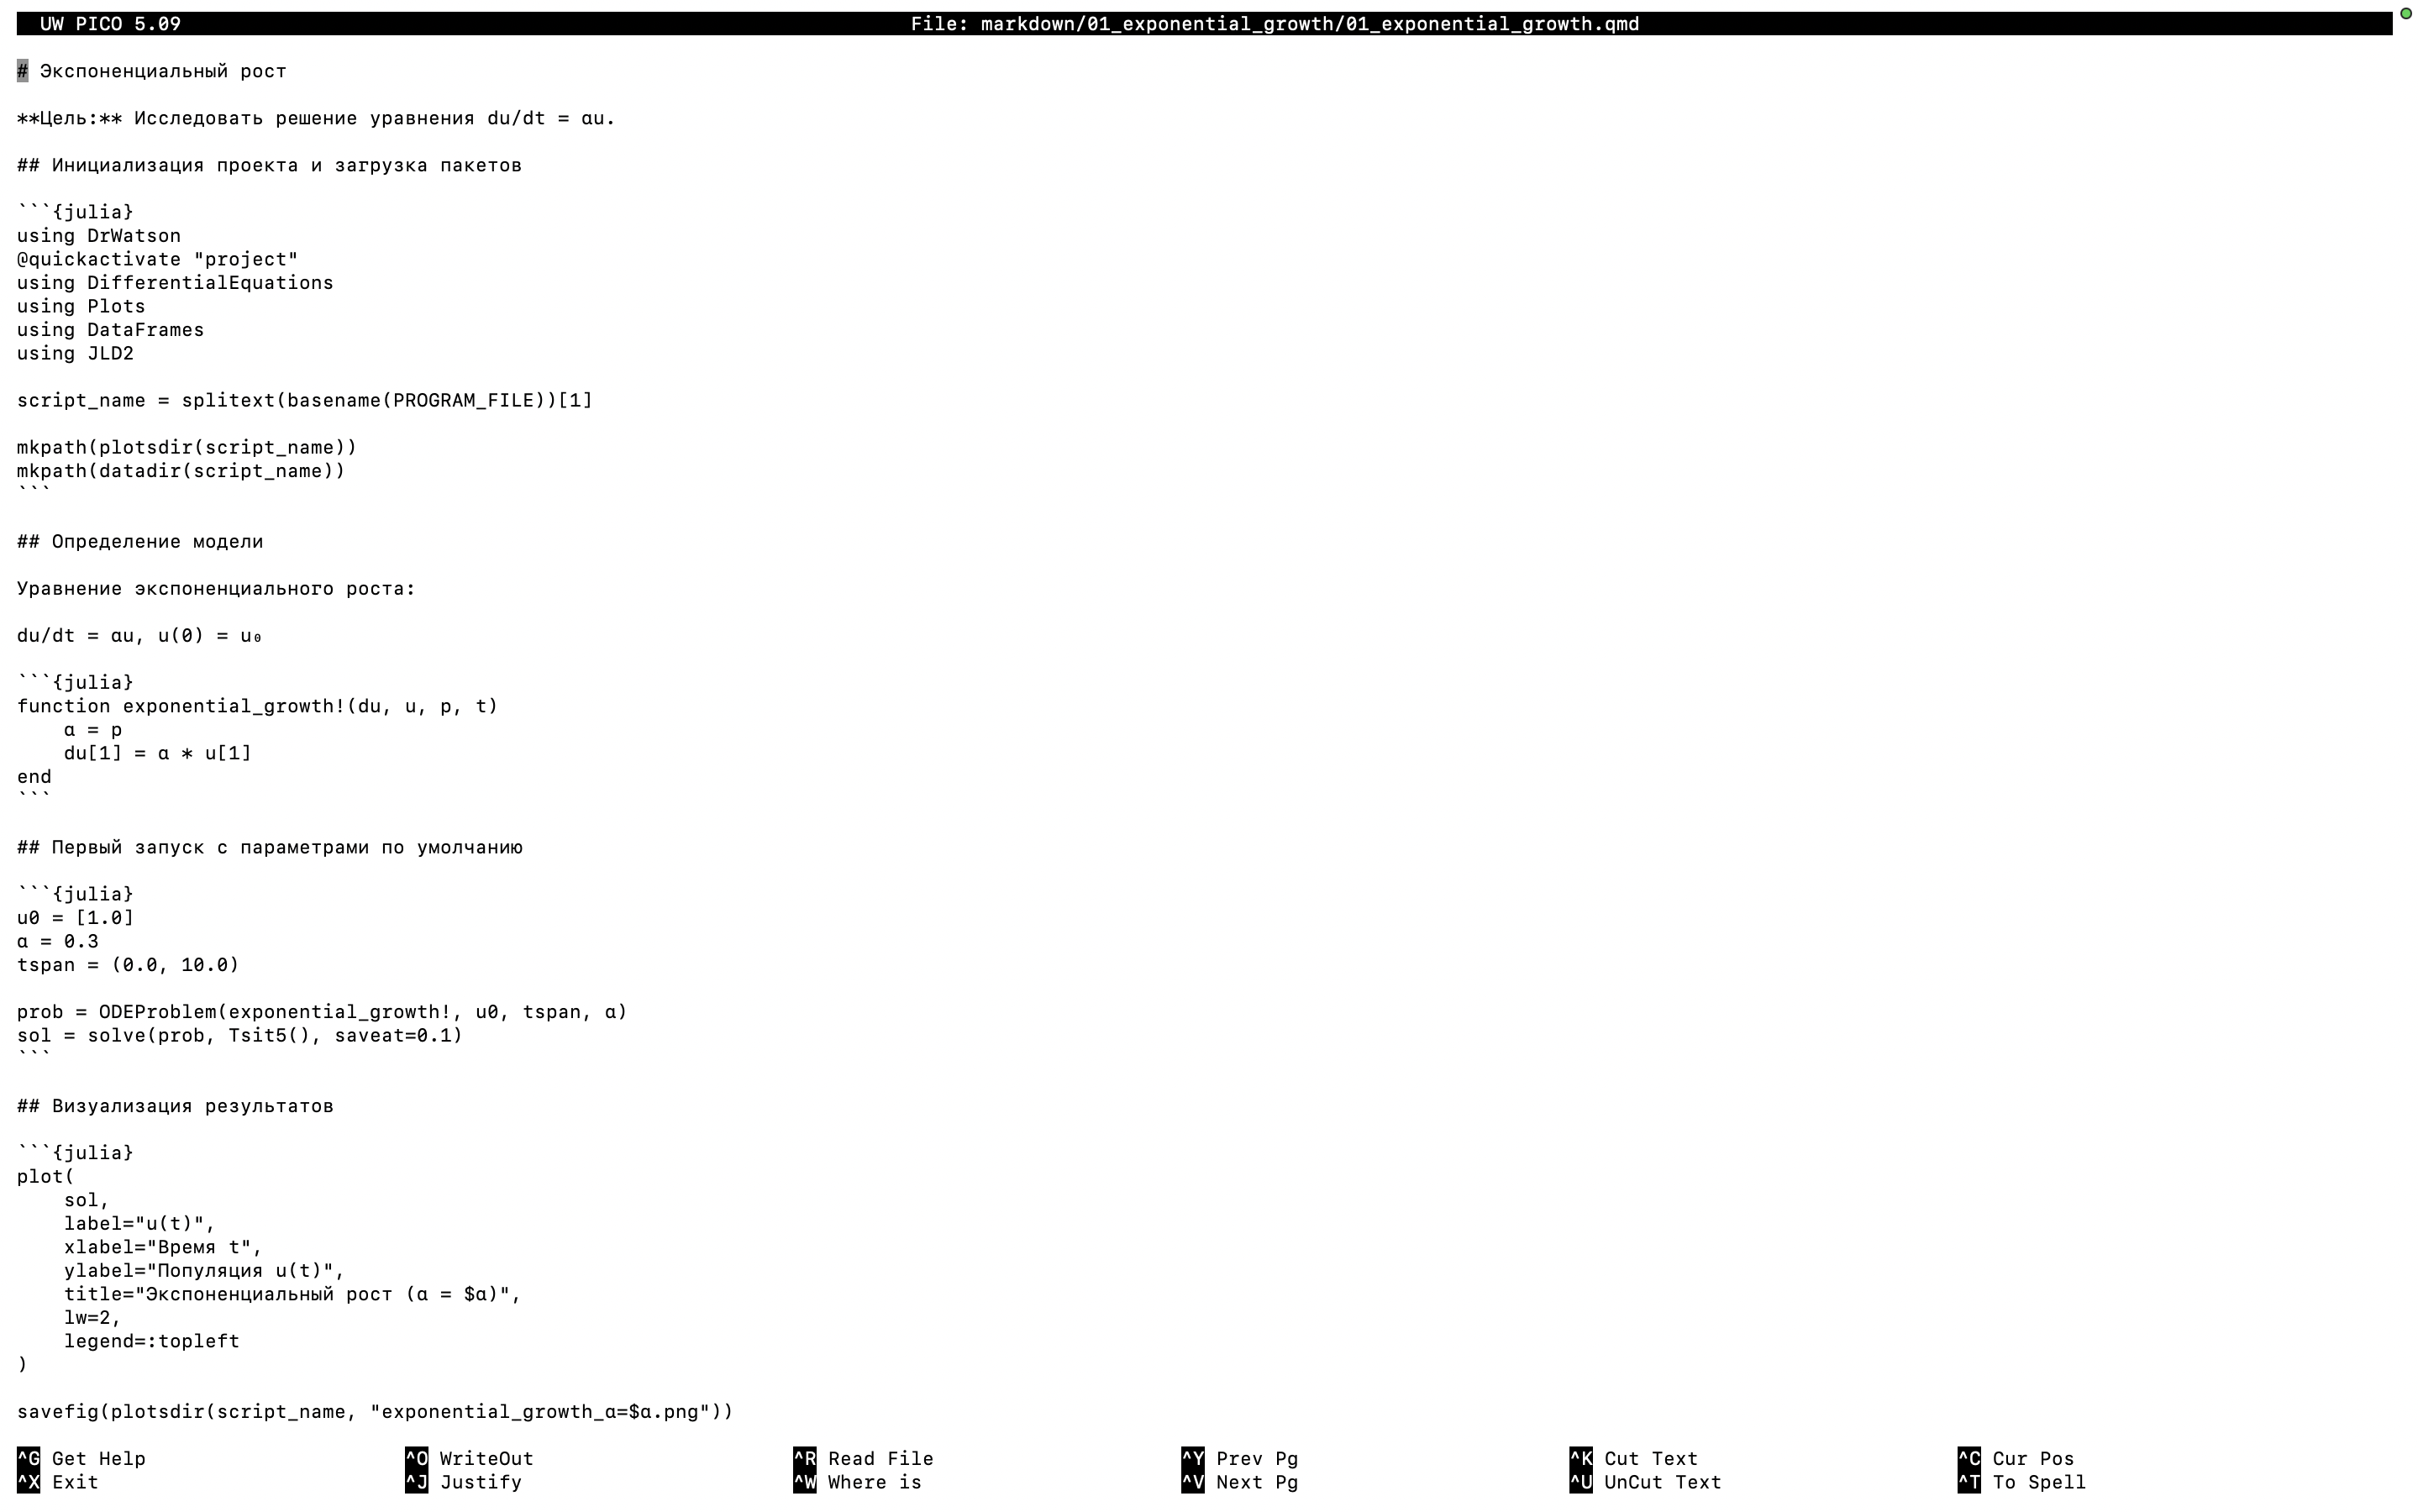
\includegraphics[width=0.7\linewidth,height=\textheight,keepaspectratio]{image/10.png}

}

\caption{\label{fig-010}Литературный документ}

\end{figure}%
\end{frame}

\begin{frame}{Генерация форматов}
\protect\phantomsection\label{ux433ux435ux43dux435ux440ux430ux446ux438ux44f-ux444ux43eux440ux43cux430ux442ux43eux432}
Из литературного кода сгенерированы производные файлы:

\begin{itemize}[<+->]
\tightlist
\item
  Julia-скрипт
\item
  Quarto-документ
\item
  Jupyter Notebook
\end{itemize}

\begin{figure}

\centering{

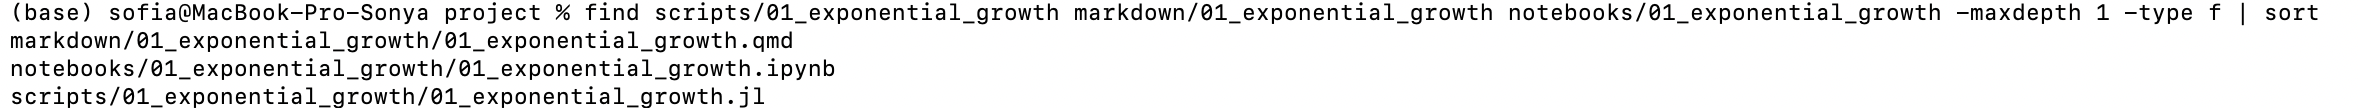
\includegraphics[width=0.7\linewidth,height=\textheight,keepaspectratio]{image/11.png}

}

\caption{\label{fig-011}Генерация производных форматов}

\end{figure}%
\end{frame}

\section{Параметрическое
исследование}\label{ux43fux430ux440ux430ux43cux435ux442ux440ux438ux447ux435ux441ux43aux43eux435-ux438ux441ux441ux43bux435ux434ux43eux432ux430ux43dux438ux435}

\begin{frame}{Исследование параметра \(\alpha\)}
\protect\phantomsection\label{ux438ux441ux441ux43bux435ux434ux43eux432ux430ux43dux438ux435-ux43fux430ux440ux430ux43cux435ux442ux440ux430-alpha}
Рассмотрены значения:

\[
\alpha \in \{0.1,\;0.3,\;0.5,\;0.8,\;1.0\}
\]

При увеличении \(\alpha\) скорость роста увеличивается.

\begin{figure}

\centering{

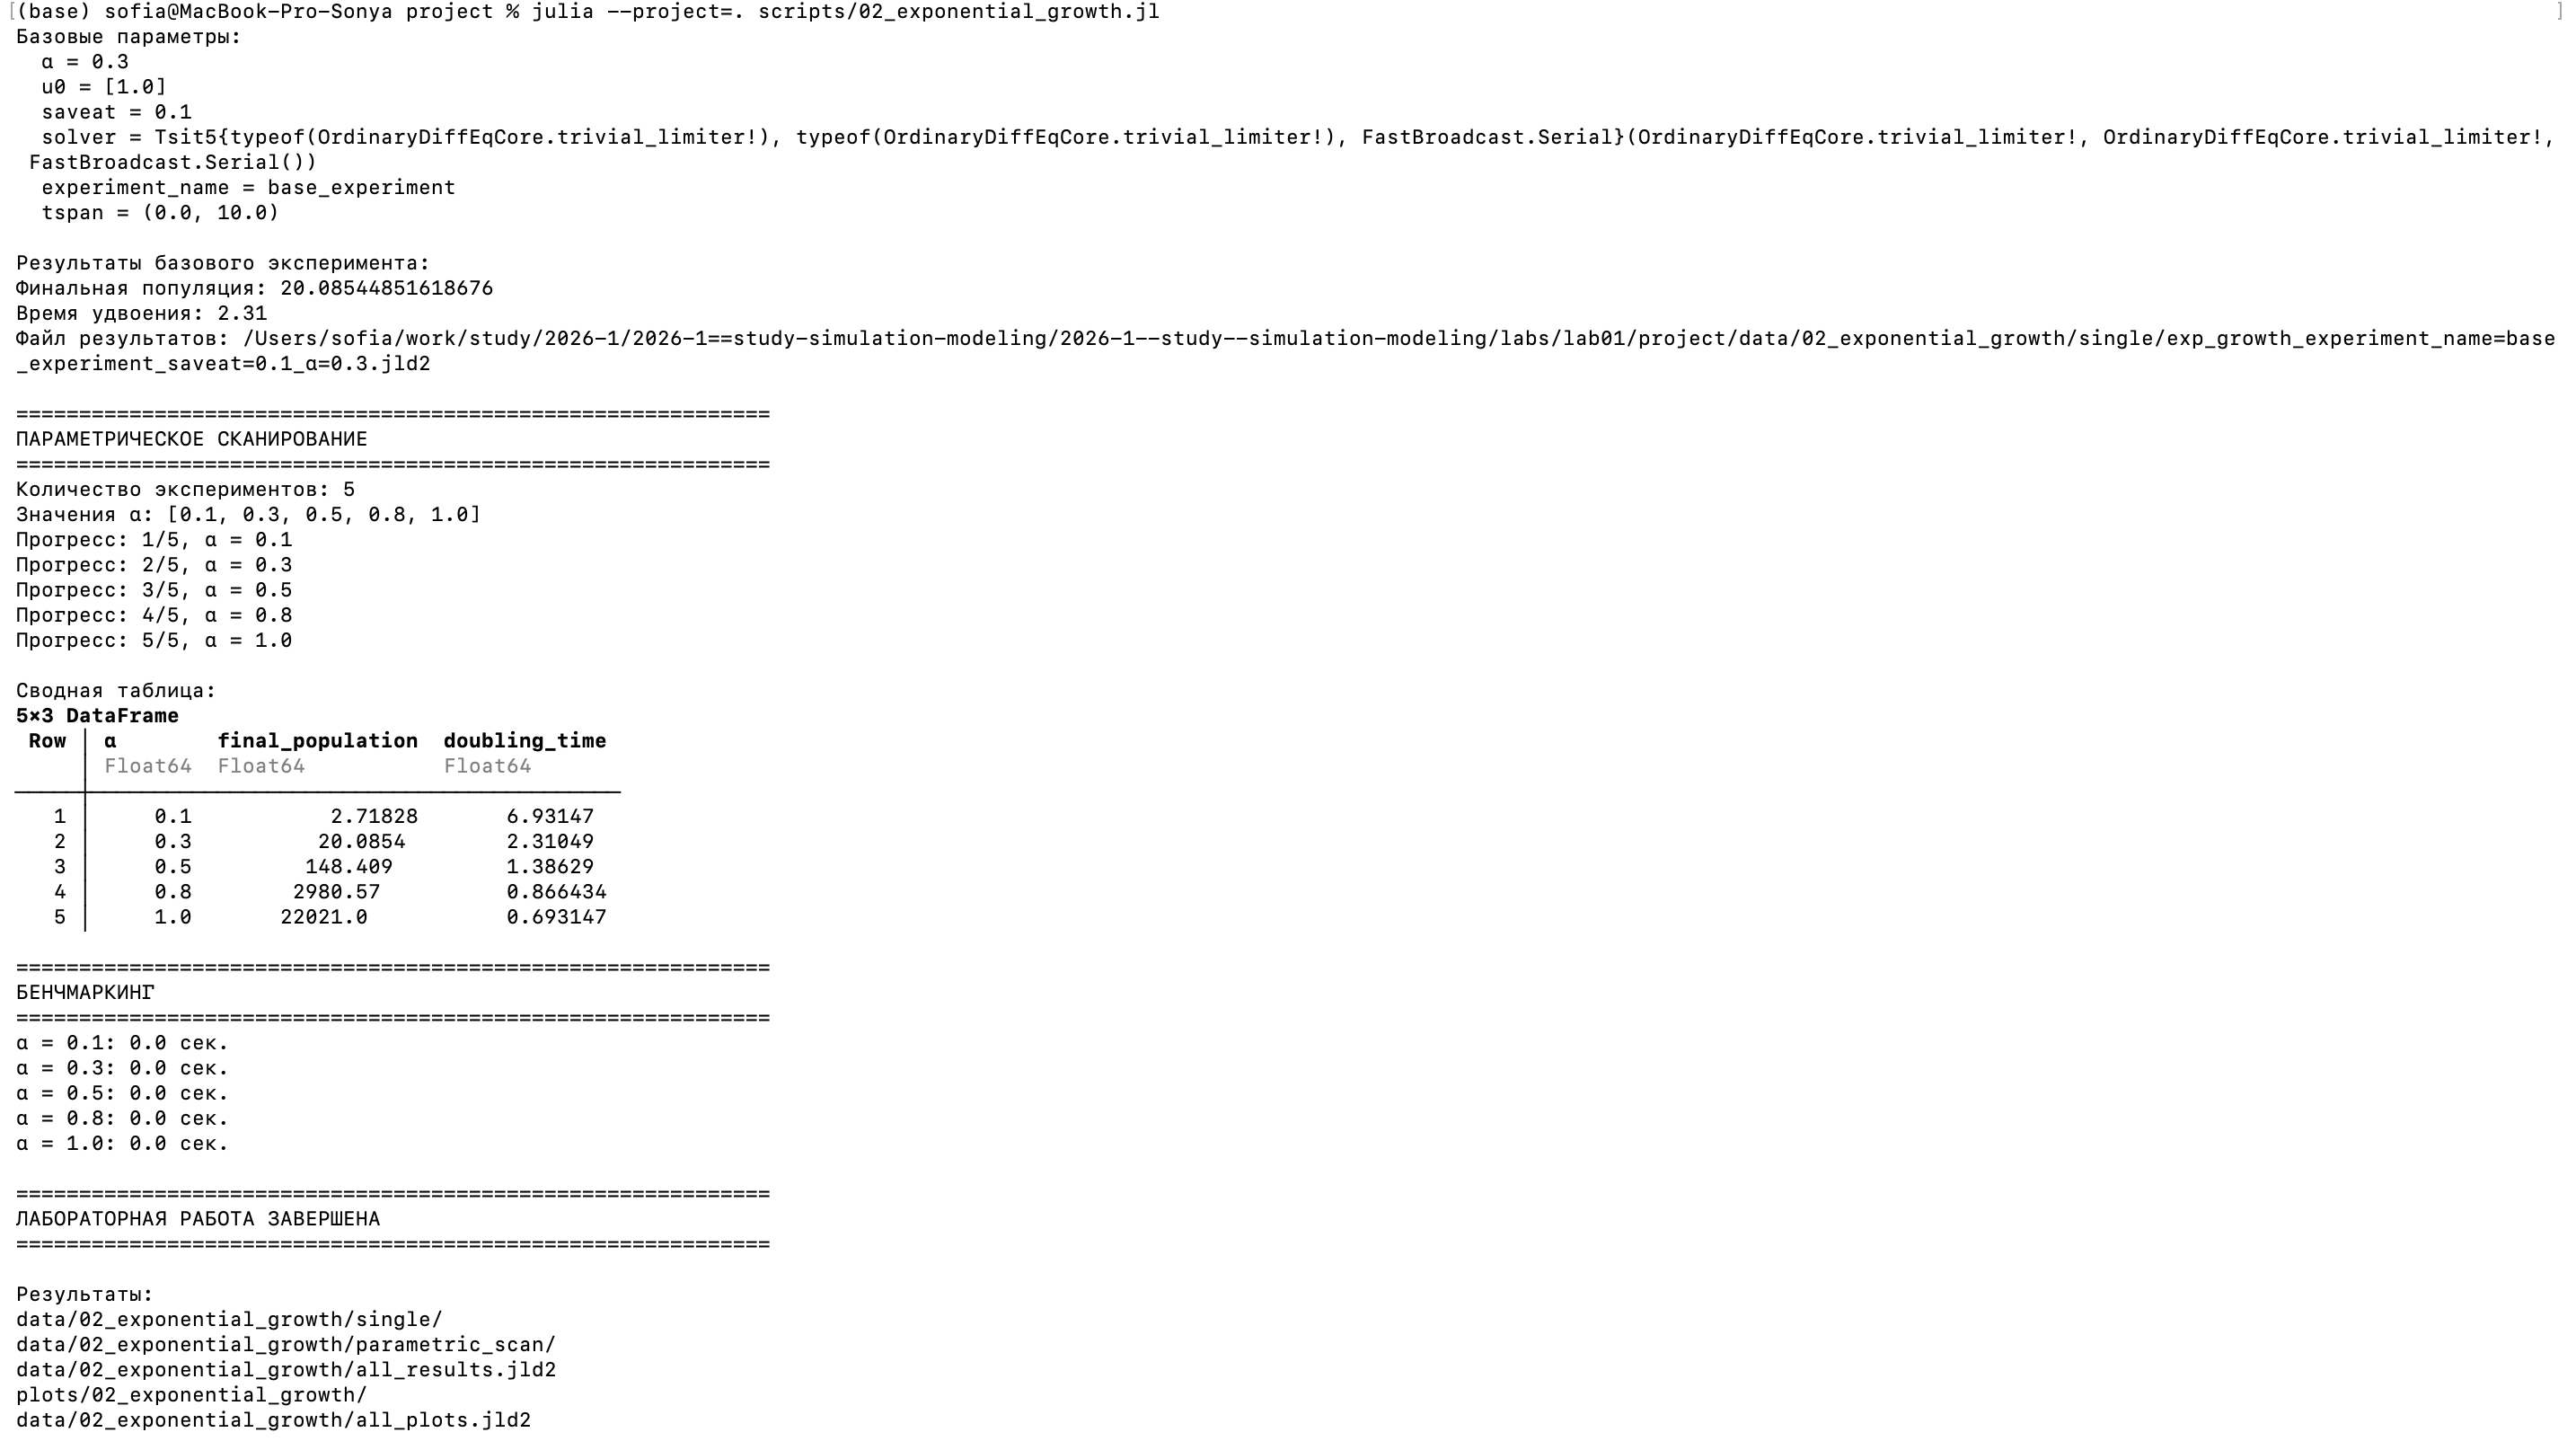
\includegraphics[width=0.7\linewidth,height=\textheight,keepaspectratio]{image/12.png}

}

\caption{\label{fig-012}Параметрическое сканирование}

\end{figure}%
\end{frame}

\begin{frame}{Сравнение траекторий}
\protect\phantomsection\label{ux441ux440ux430ux432ux43dux435ux43dux438ux435-ux442ux440ux430ux435ux43aux442ux43eux440ux438ux439}
\begin{itemize}[<+->]
\tightlist
\item
  \(\alpha=0.1\) --- наиболее медленный рост
\item
  \(\alpha=1.0\) --- наиболее быстрый рост
\item
  увеличение \(\alpha\) ускоряет развитие модели
\end{itemize}

\begin{figure}

\centering{

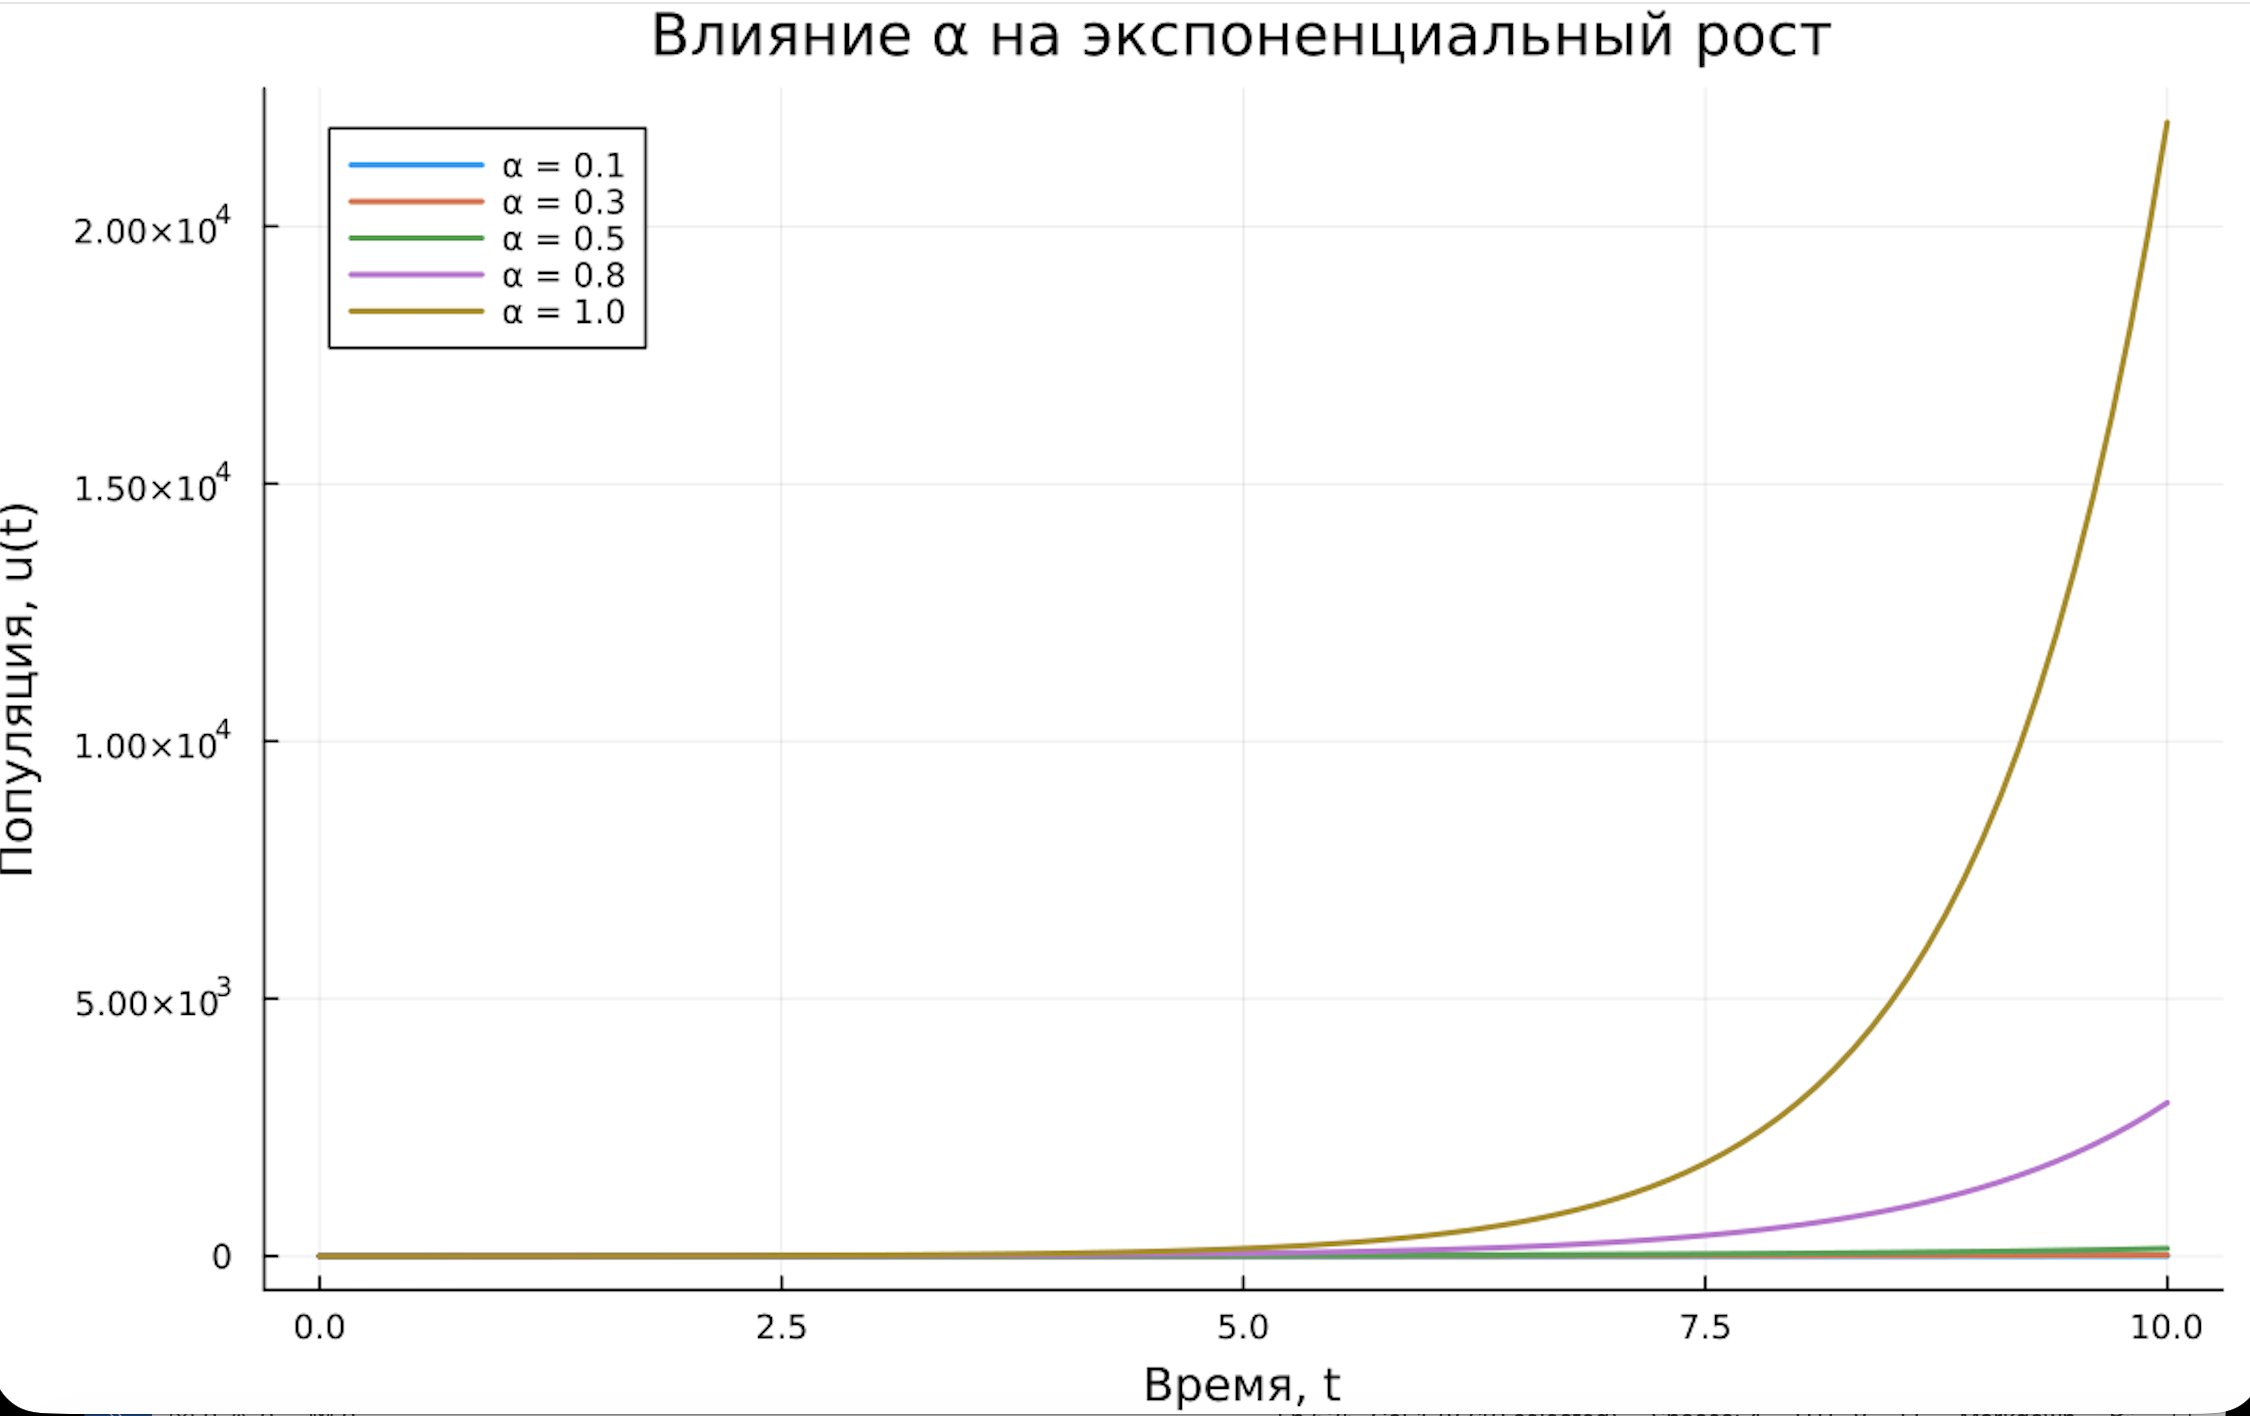
\includegraphics[width=0.7\linewidth,height=\textheight,keepaspectratio]{image/13.png}

}

\caption{\label{fig-013}Сравнение траекторий}

\end{figure}%
\end{frame}

\begin{frame}{Время удвоения от \(\alpha\)}
\protect\phantomsection\label{ux432ux440ux435ux43cux44f-ux443ux434ux432ux43eux435ux43dux438ux44f-ux43eux442-alpha}
Теоретическая зависимость:

\[
T_2=\frac{\ln 2}{\alpha}
\]

При увеличении \(\alpha\) время удвоения уменьшается.

\begin{figure}

\centering{

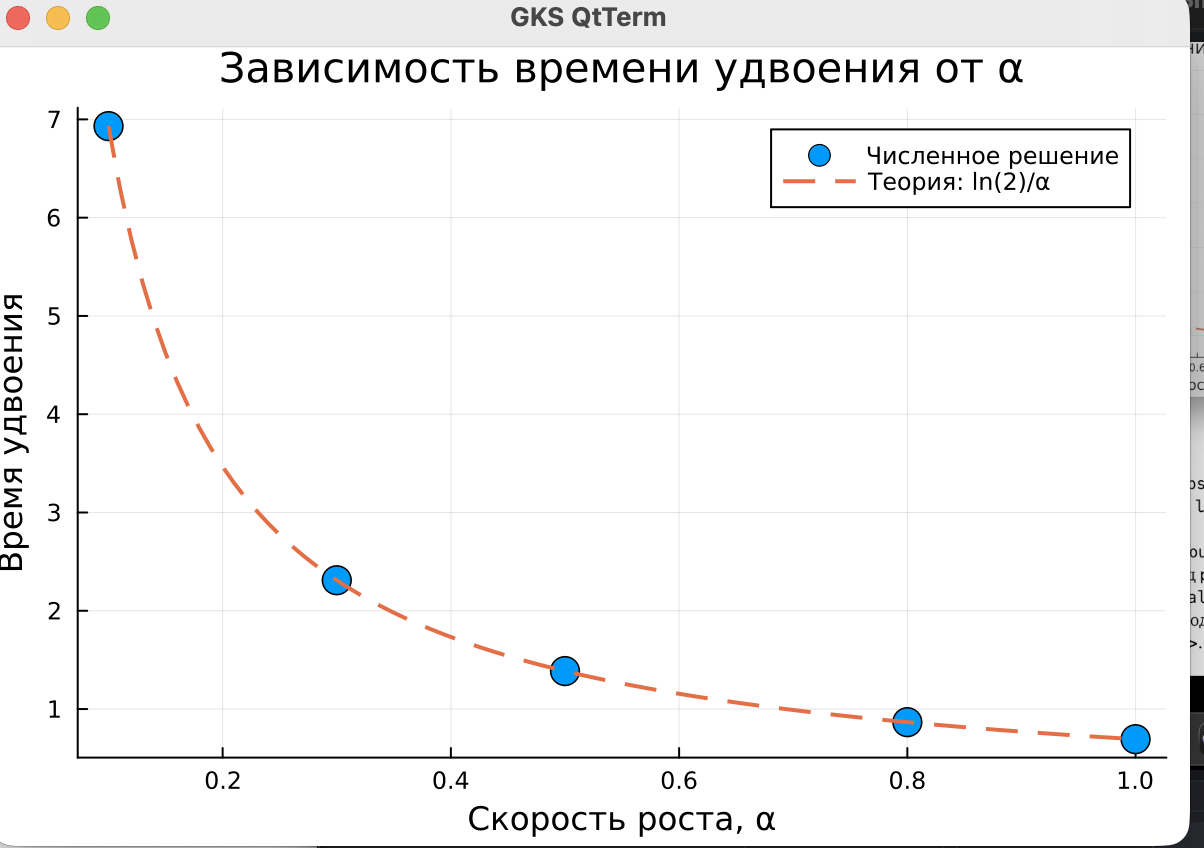
\includegraphics[width=0.7\linewidth,height=\textheight,keepaspectratio]{image/14.png}

}

\caption{\label{fig-014}Зависимость времени удвоения от \(\alpha\)}

\end{figure}%
\end{frame}

\section{Бенчмаркинг}\label{ux431ux435ux43dux447ux43cux430ux440ux43aux438ux43dux433}

\begin{frame}[fragile]{Время вычислений}
\protect\phantomsection\label{ux432ux440ux435ux43cux44f-ux432ux44bux447ux438ux441ux43bux435ux43dux438ux439}
Для различных значений \(\alpha\) выполнено измерение времени численного
решения с помощью пакета \texttt{BenchmarkTools}.

\begin{figure}

\centering{

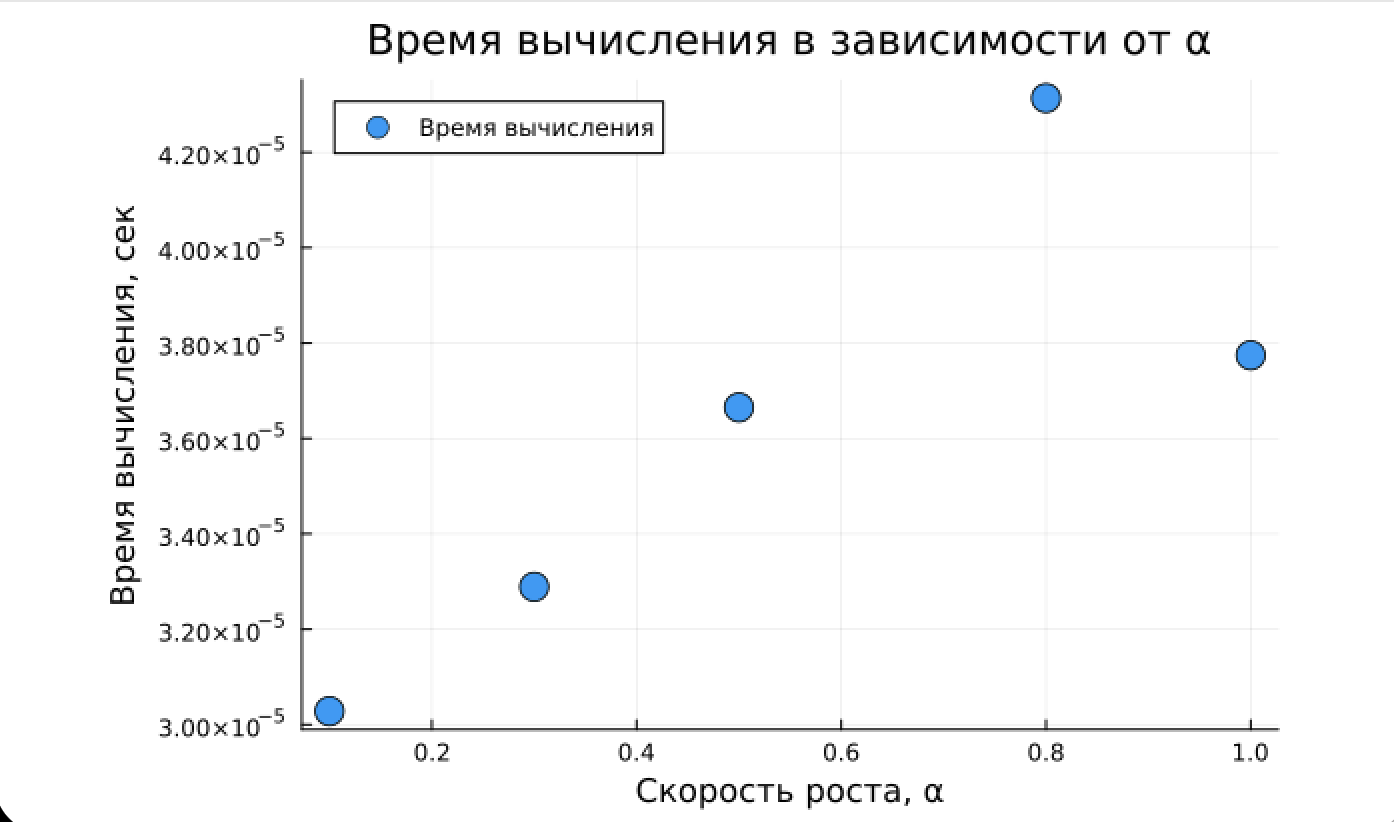
\includegraphics[width=0.7\linewidth,height=\textheight,keepaspectratio]{image/15.png}

}

\caption{\label{fig-015}График времени вычисления}

\end{figure}%
\end{frame}

\section{Jupyter и Quarto}\label{jupyter-ux438-quarto}

\begin{frame}{Jupyter Notebook}
\protect\phantomsection\label{jupyter-notebook}
Подготовлены два ноутбука:

\begin{itemize}[<+->]
\tightlist
\item
  01\_exponential\_growth.ipynb
\item
  02\_exponential\_growth.ipynb
\end{itemize}

\begin{figure}

\centering{

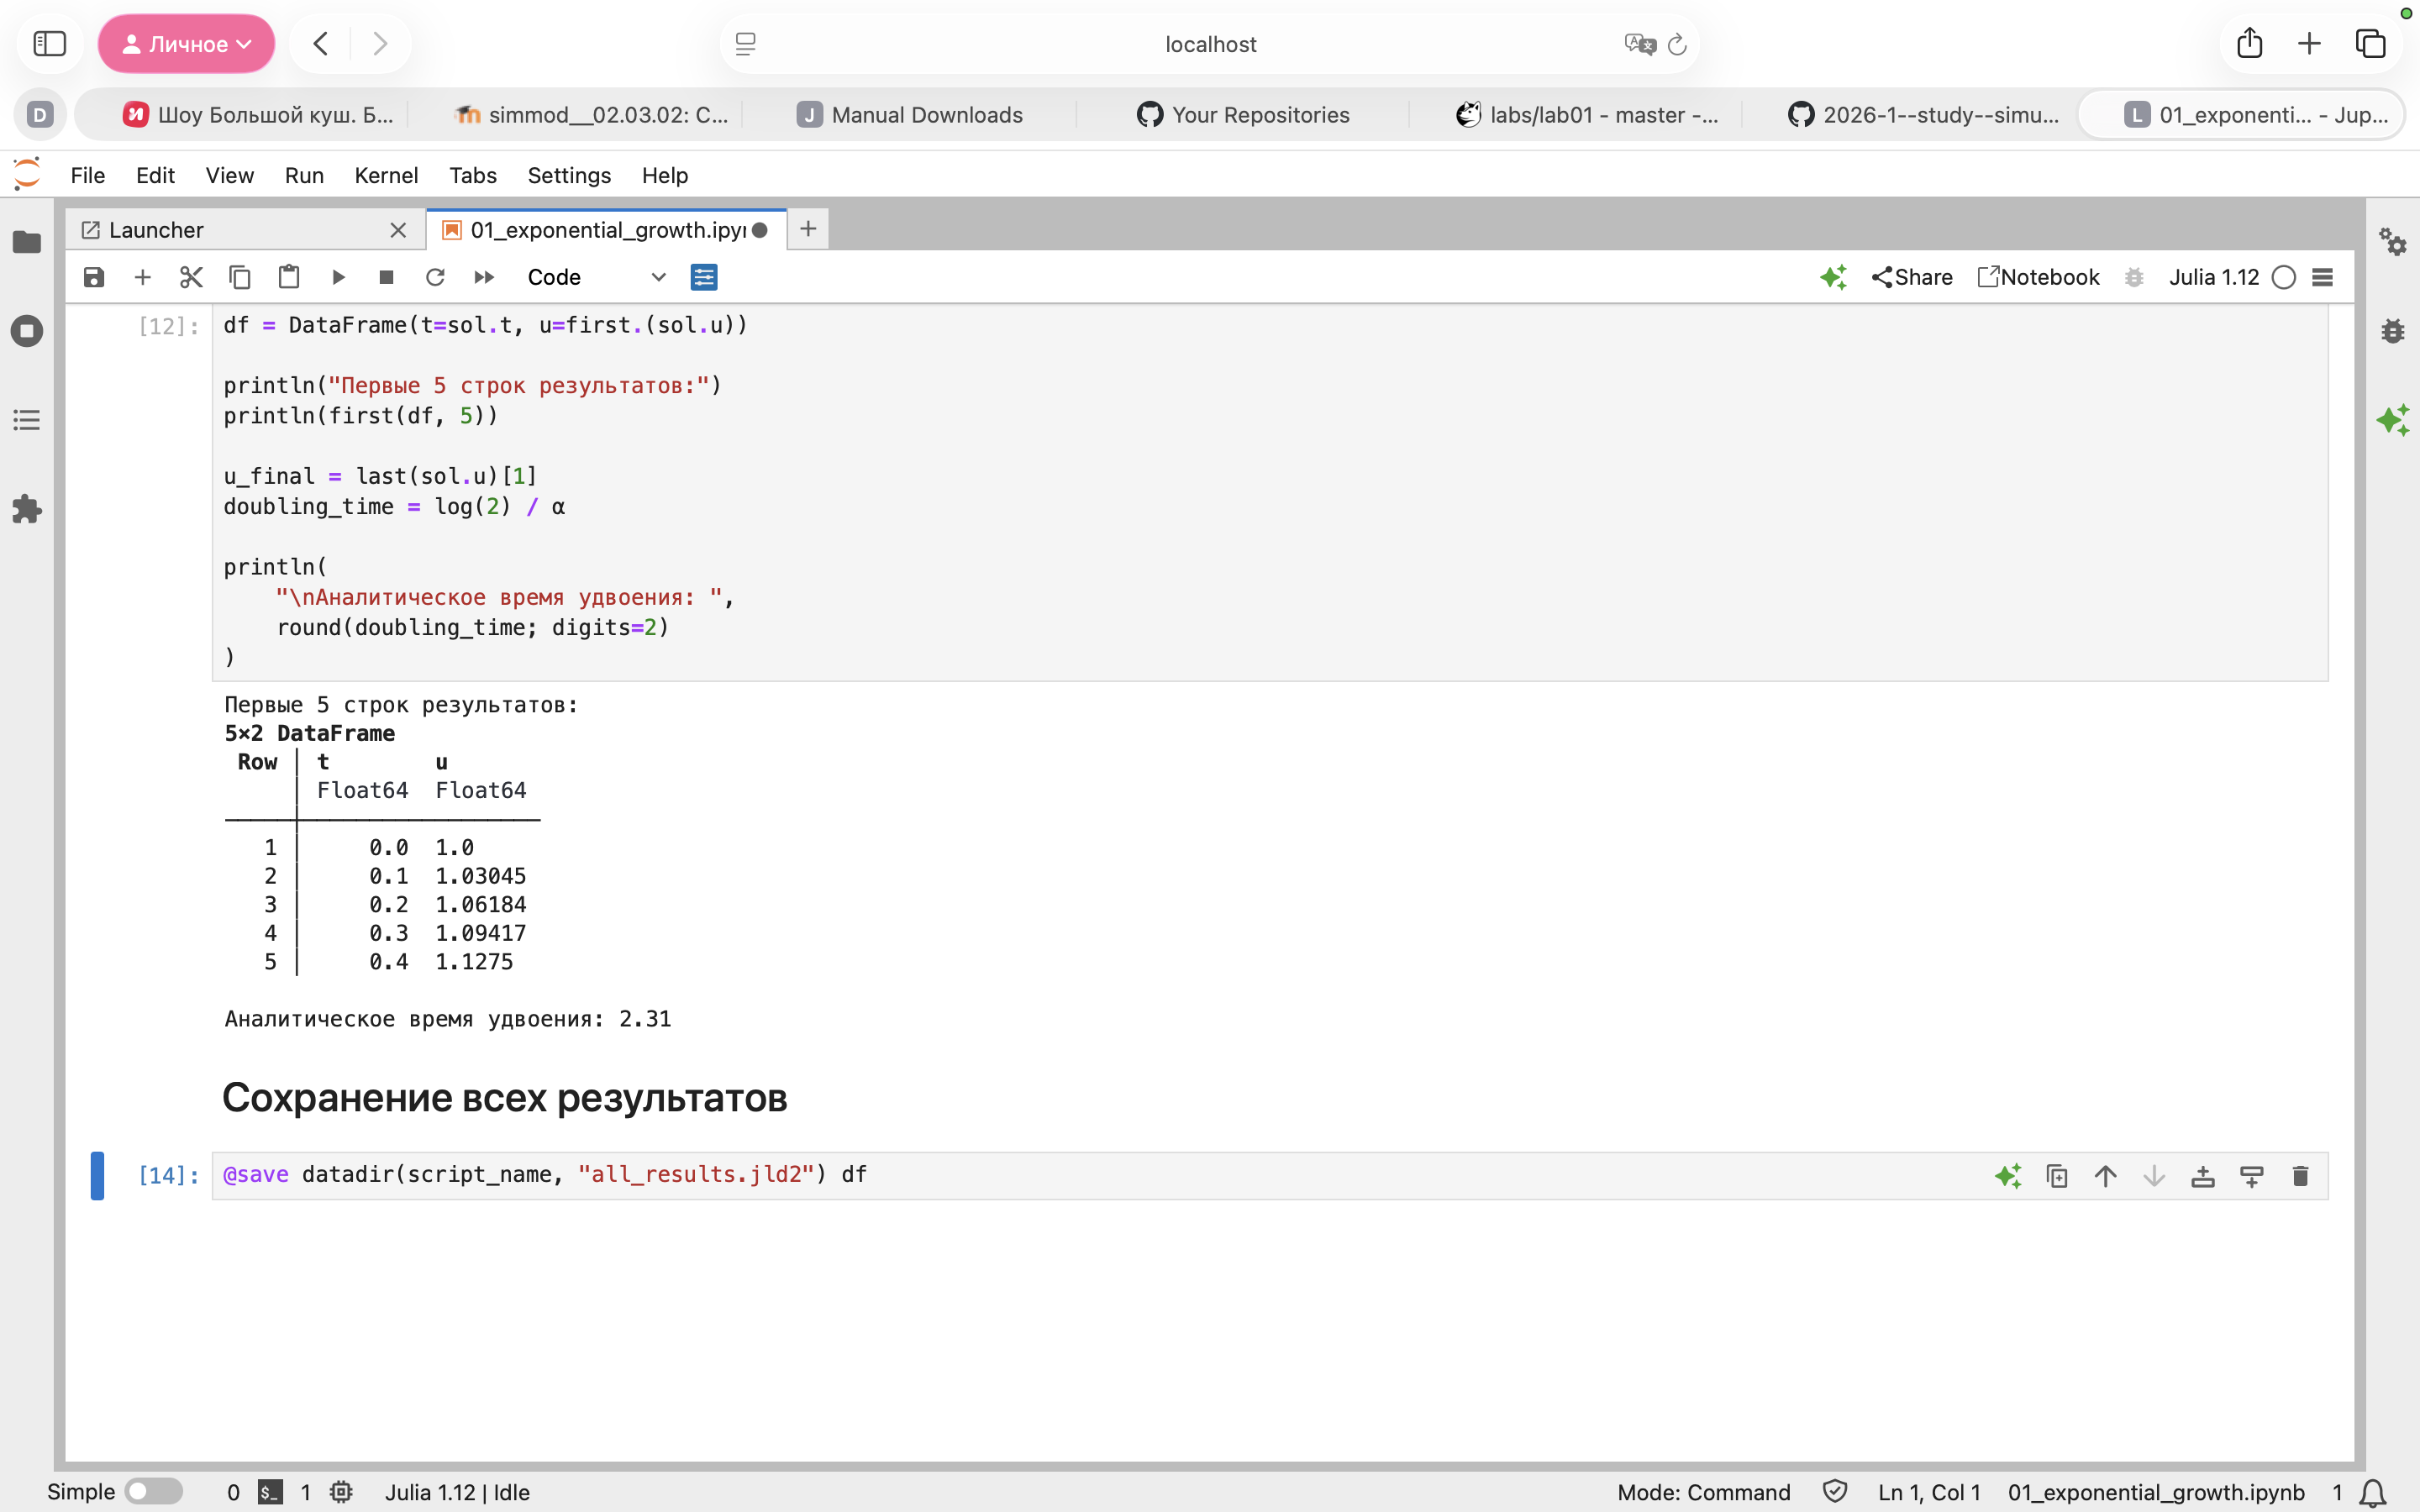
\includegraphics[width=0.7\linewidth,height=\textheight,keepaspectratio]{image/16.png}

}

\caption{\label{fig-016}Результат выполнения Jupyter Notebook}

\end{figure}%

\begin{figure}

\centering{

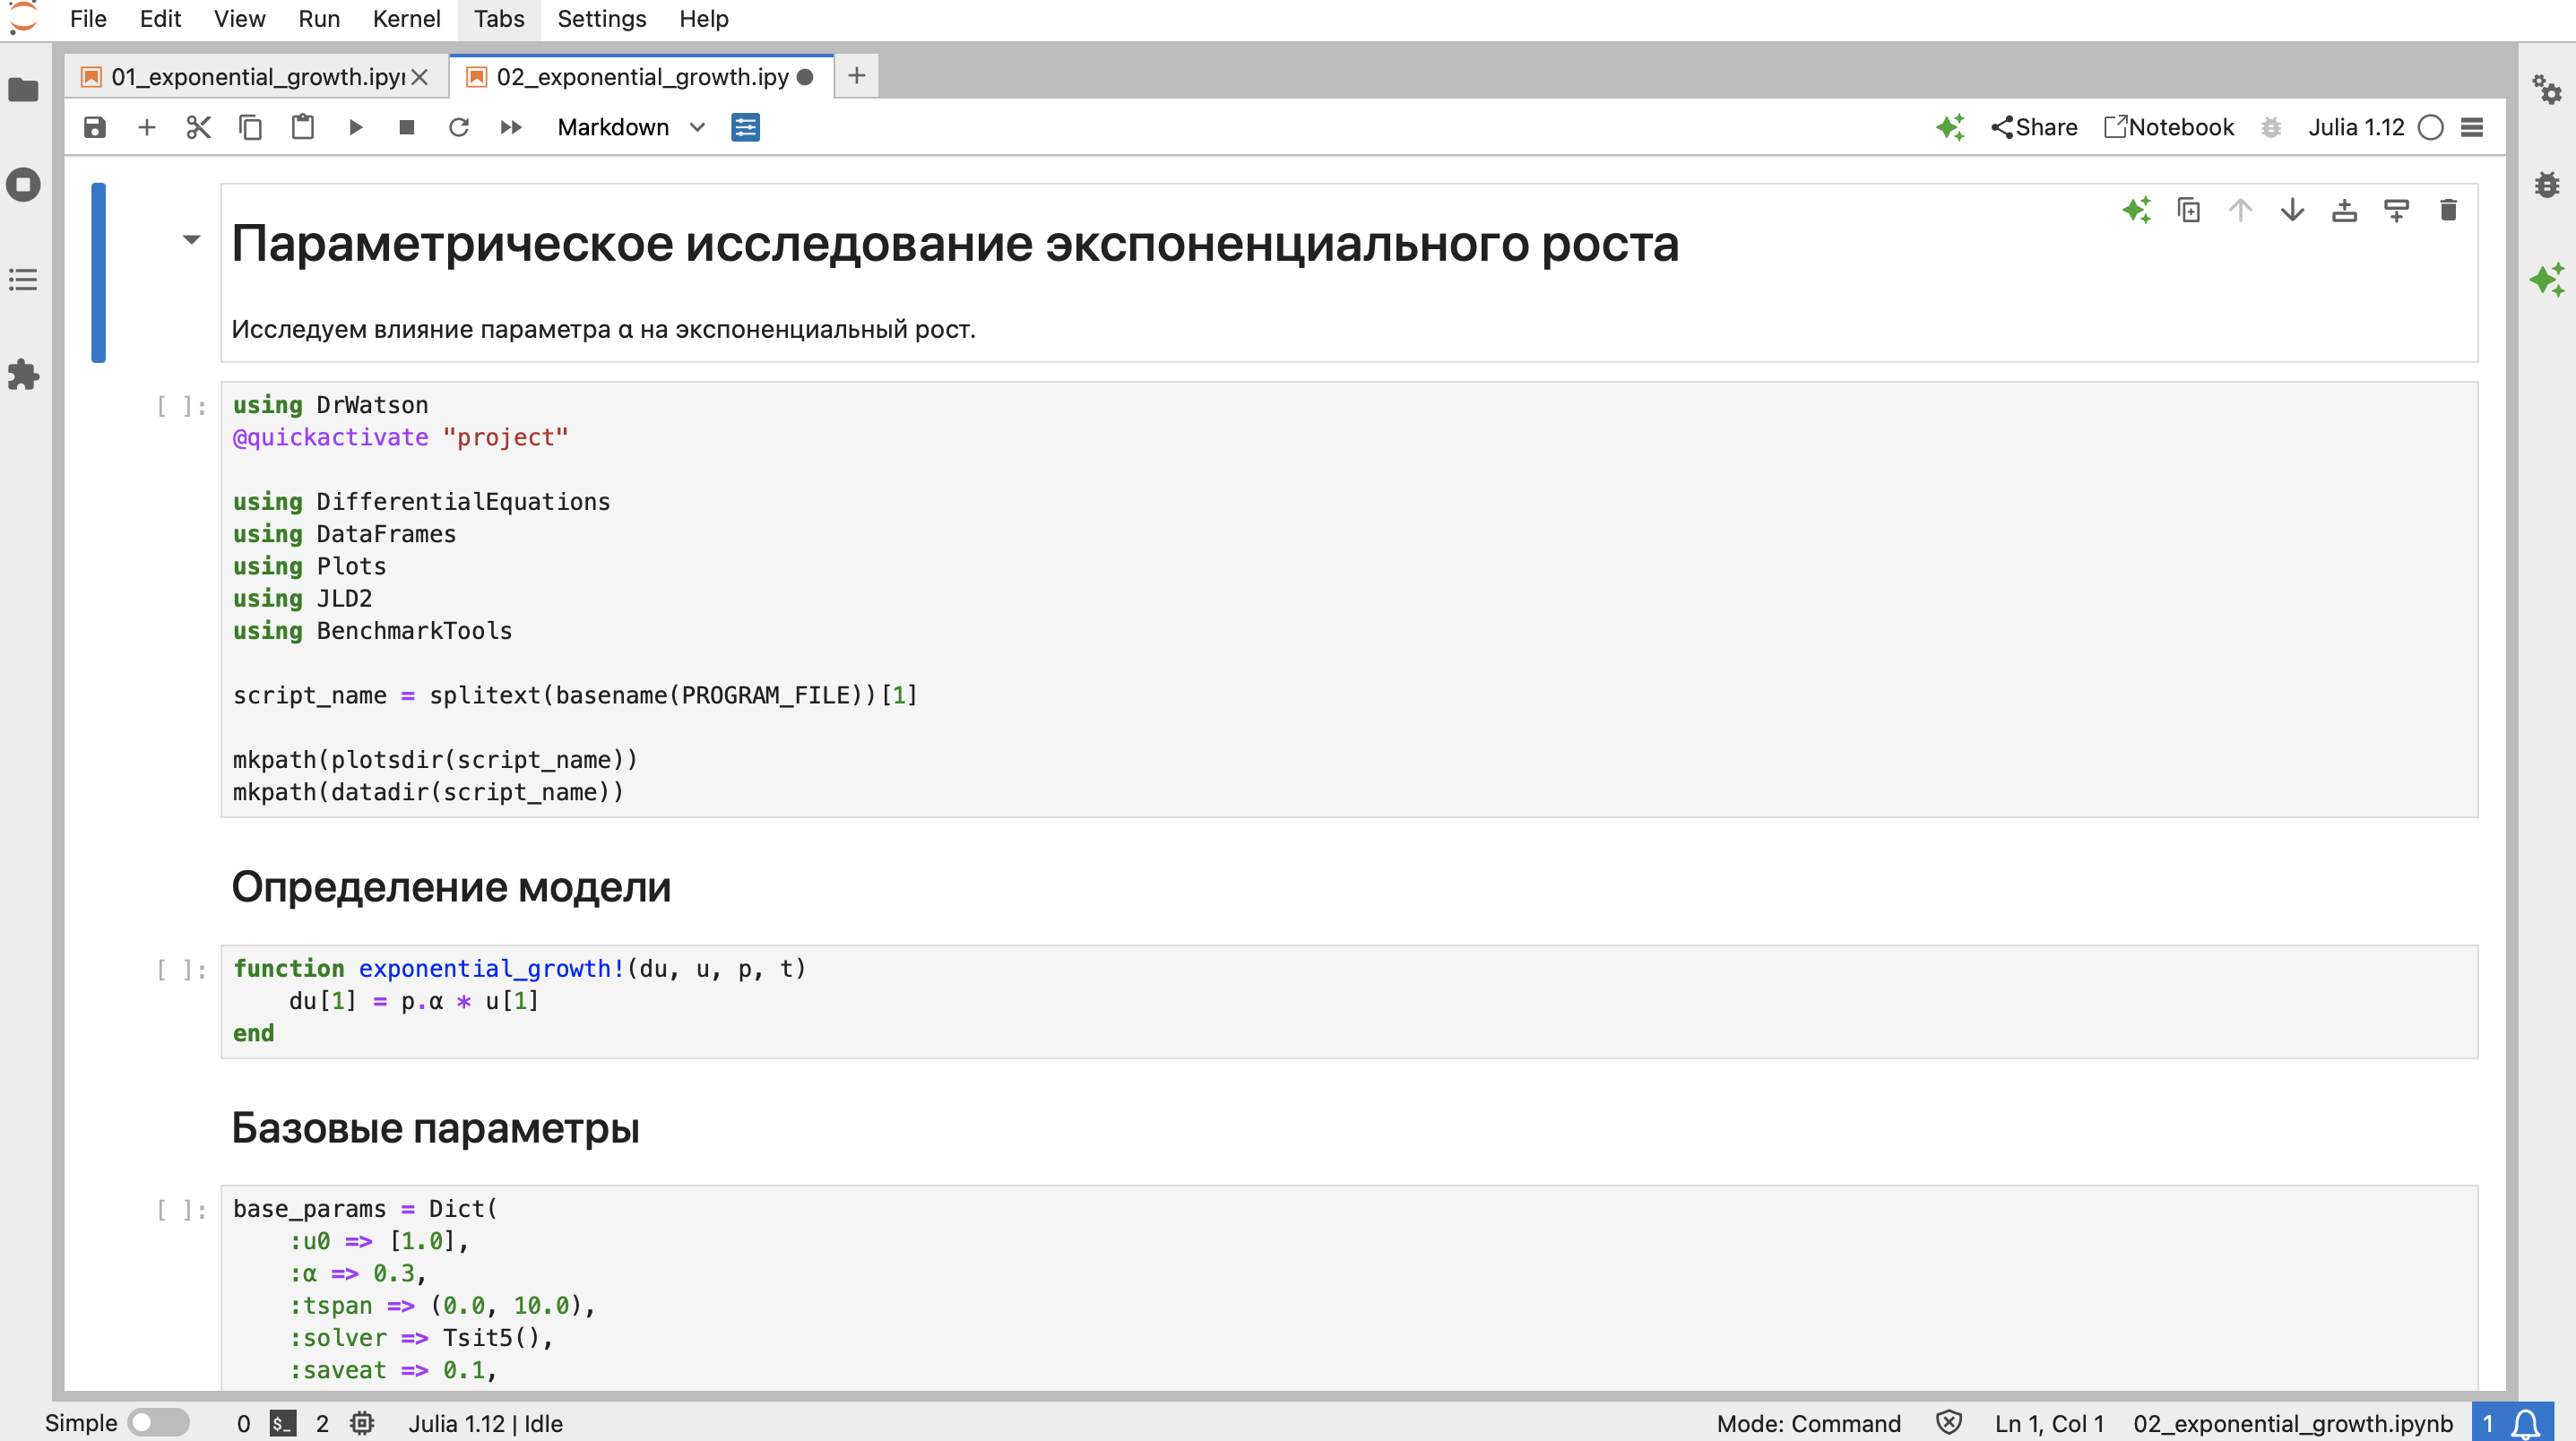
\includegraphics[width=0.7\linewidth,height=\textheight,keepaspectratio]{image/161.png}

}

\caption{\label{fig-161}Результат выполнения Jupyter Notebook}

\end{figure}%
\end{frame}

\begin{frame}[fragile]{Quarto}
\protect\phantomsection\label{quarto}
Отчёт собирается средствами Quarto с использованием Julia:

\begin{Shaded}
\begin{Highlighting}[]
\FunctionTok{engine}\KeywordTok{:}\AttributeTok{ julia}
\FunctionTok{julia}\KeywordTok{:}
\AttributeTok{  }\FunctionTok{exeflags}\KeywordTok{:}\AttributeTok{ }\KeywordTok{[}\StringTok{"{-}{-}project=../project"}\KeywordTok{]}
\end{Highlighting}
\end{Shaded}

\begin{figure}

\centering{

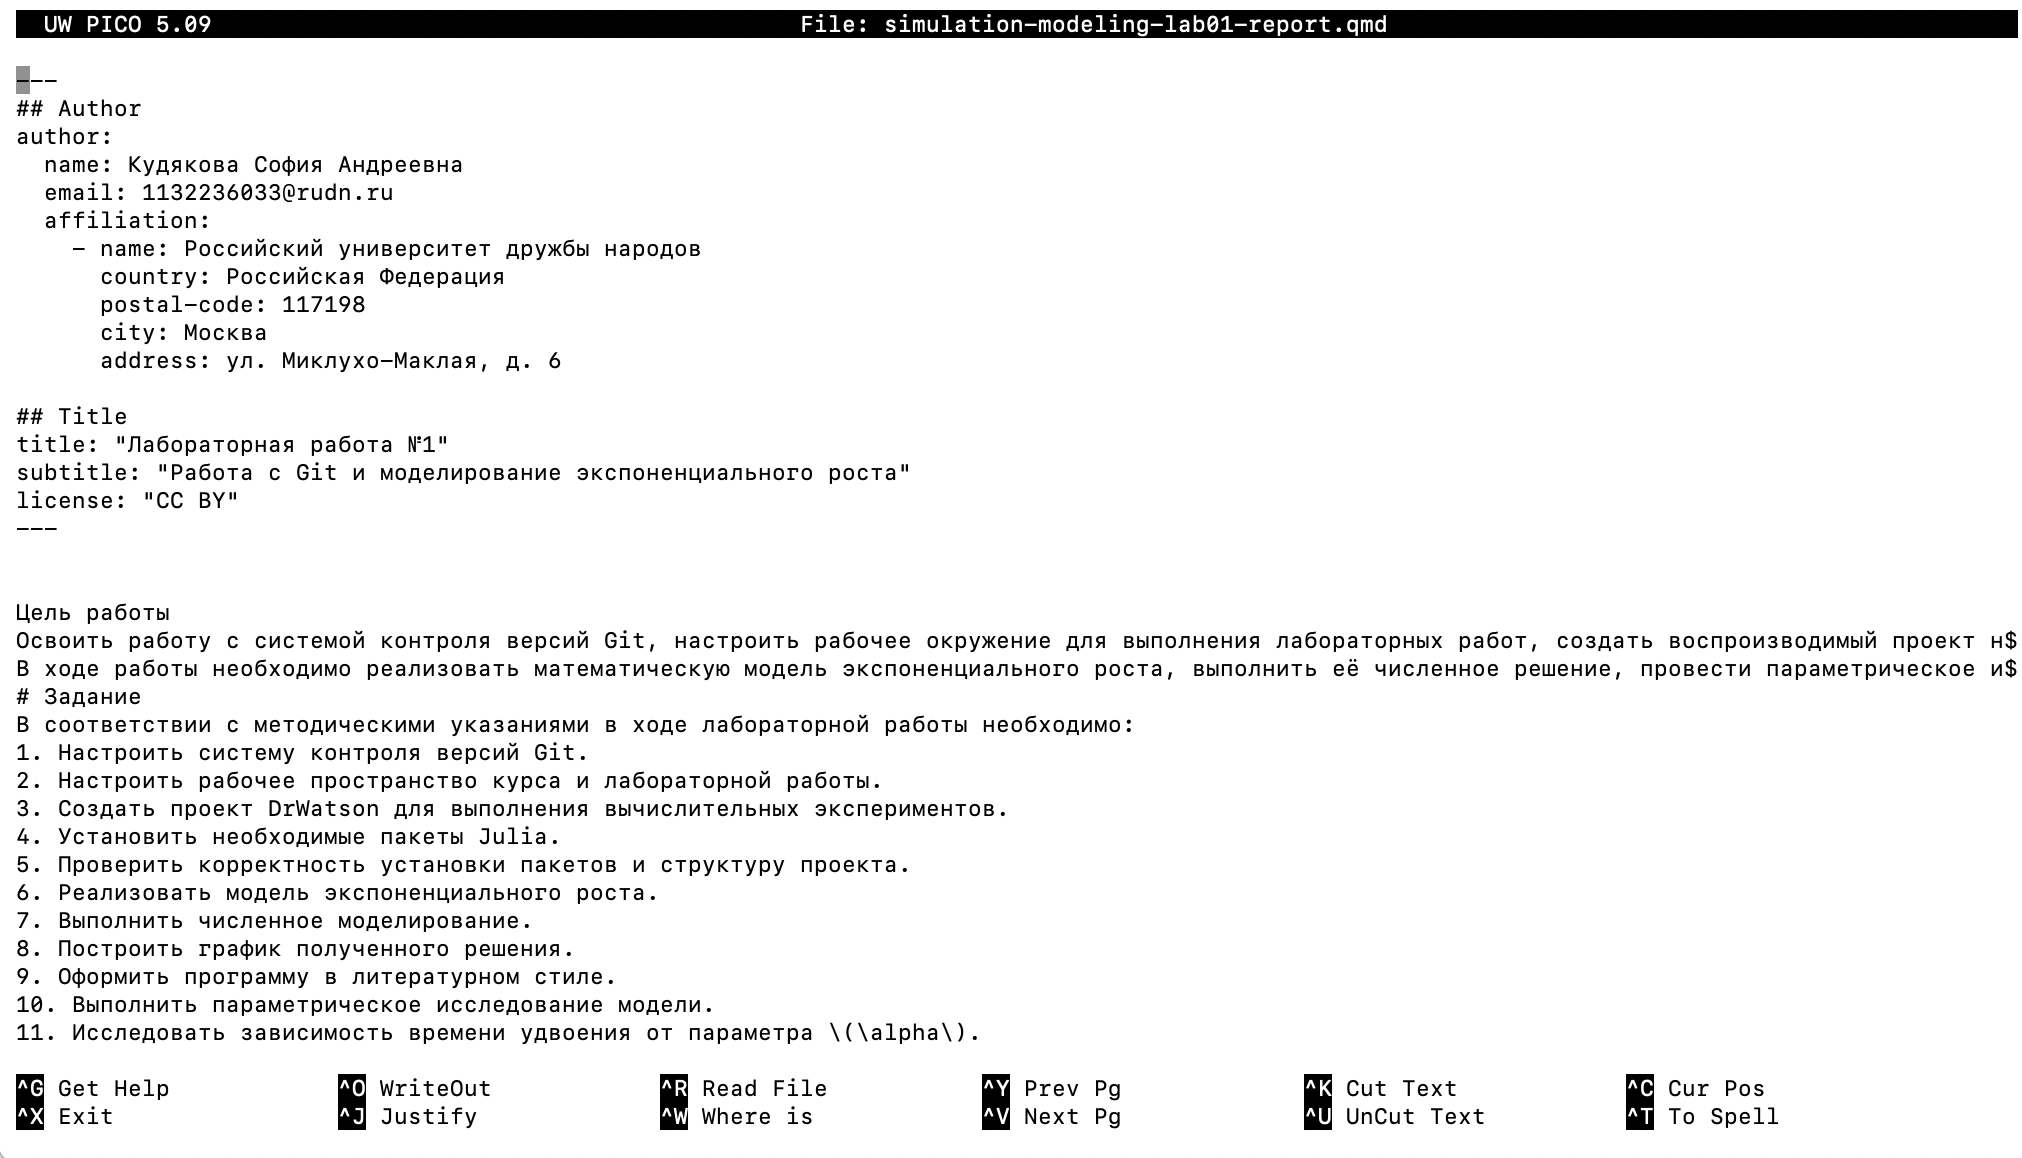
\includegraphics[width=0.7\linewidth,height=\textheight,keepaspectratio]{image/17.png}

}

\caption{\label{fig-017}Quarto}

\end{figure}%
\end{frame}

\begin{frame}[fragile]{Итоговая структура}
\protect\phantomsection\label{ux438ux442ux43eux433ux43eux432ux430ux44f-ux441ux442ux440ux443ux43aux442ux443ux440ux430}
Сформирована итоговая структура лабораторной работы:
\texttt{presentation/}, \texttt{project/}, \texttt{report/}.

\begin{figure}

\centering{

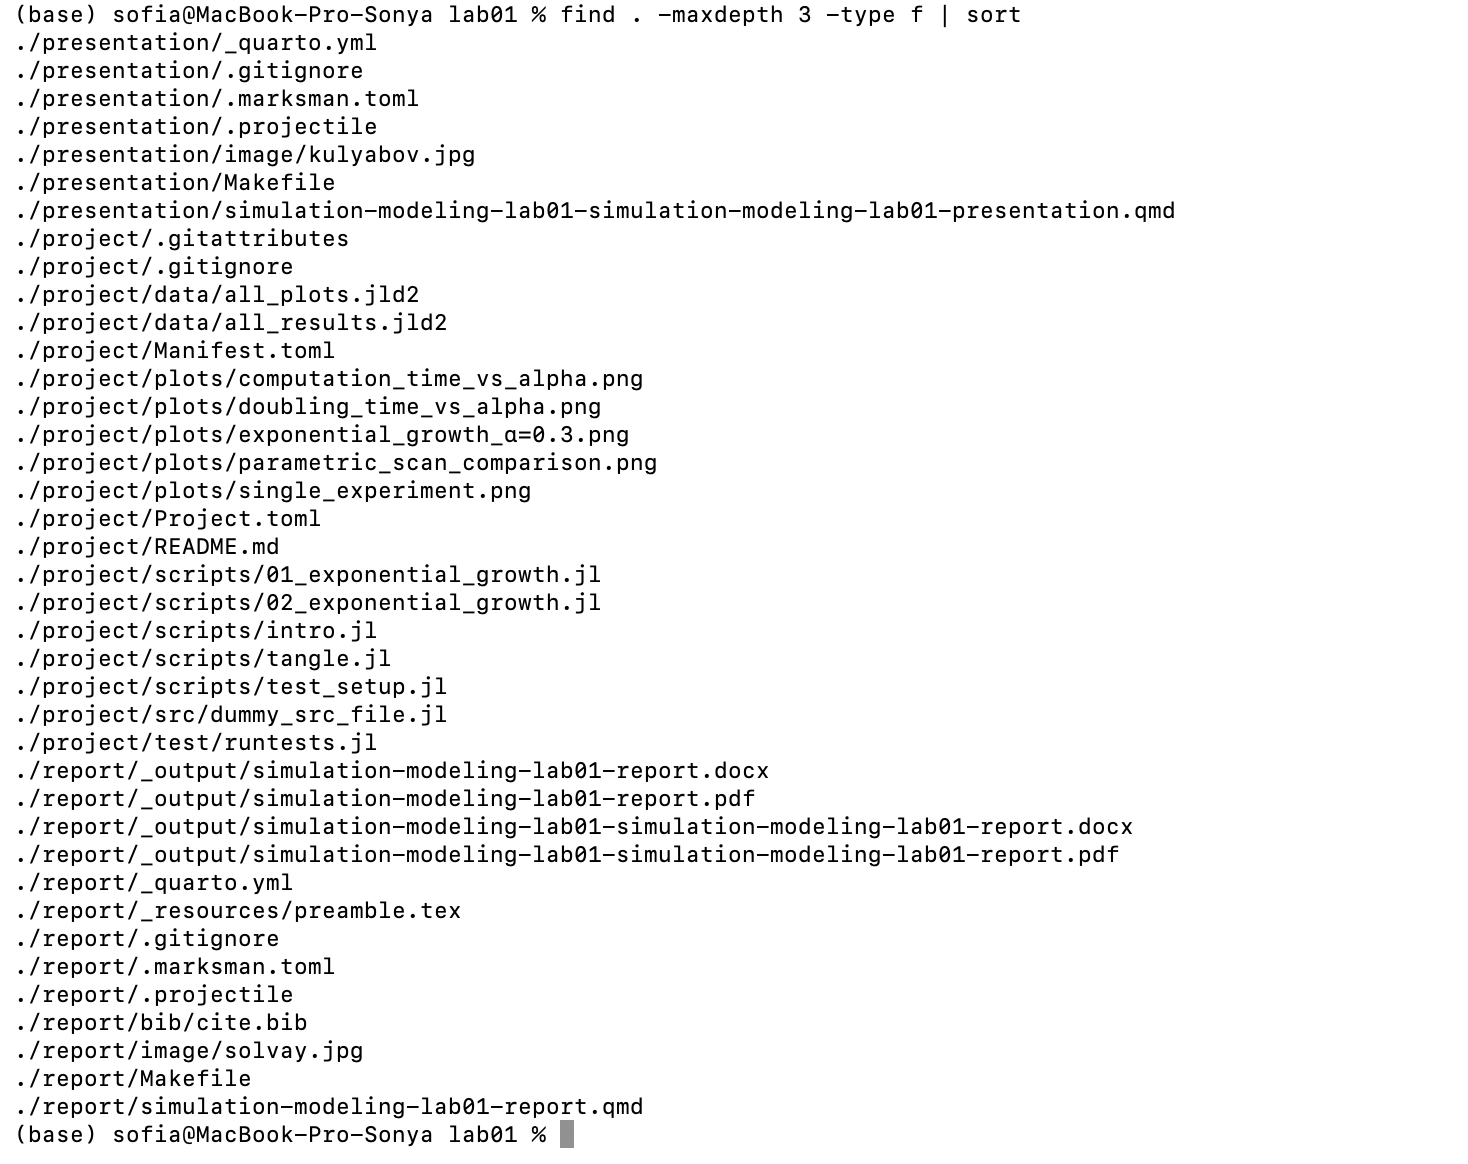
\includegraphics[width=0.7\linewidth,height=\textheight,keepaspectratio]{image/18.png}

}

\caption{\label{fig-018}Итоговая структура лабораторной работы}

\end{figure}%
\end{frame}

\section{Результаты}\label{ux440ux435ux437ux443ux43bux44cux442ux430ux442ux44b}

\begin{frame}{Итог}
\protect\phantomsection\label{ux438ux442ux43eux433}
\begin{itemize}[<+->]
\tightlist
\item
  Настроены Git и SSH
\item
  Создан проект DrWatson
\item
  Реализована модель экспоненциального роста
\item
  Проведено параметрическое исследование
\item
  Исследовано время удвоения
\item
  Выполнен бенчмаркинг
\item
  Подготовлены Julia, Jupyter Notebook и Quarto
\end{itemize}
\end{frame}

\begin{frame}{Главное}
\protect\phantomsection\label{ux433ux43bux430ux432ux43dux43eux435}
Модель экспоненциального роста успешно реализована и исследована.

Получена зависимость:

\[
T_2=\frac{\ln 2}{\alpha}
\]

Увеличение \(\alpha\) приводит к уменьшению времени удвоения.
\end{frame}




\end{document}
